\documentclass[]{article}
\usepackage{lmodern}
\usepackage{amssymb,amsmath}
\usepackage{ifxetex,ifluatex}
\usepackage{fixltx2e} % provides \textsubscript
\ifnum 0\ifxetex 1\fi\ifluatex 1\fi=0 % if pdftex
  \usepackage[T1]{fontenc}
  \usepackage[utf8]{inputenc}
\else % if luatex or xelatex
  \ifxetex
    \usepackage{mathspec}
  \else
    \usepackage{fontspec}
  \fi
  \defaultfontfeatures{Ligatures=TeX,Scale=MatchLowercase}
\fi
% use upquote if available, for straight quotes in verbatim environments
\IfFileExists{upquote.sty}{\usepackage{upquote}}{}
% use microtype if available
\IfFileExists{microtype.sty}{%
\usepackage{microtype}
\UseMicrotypeSet[protrusion]{basicmath} % disable protrusion for tt fonts
}{}
\usepackage[margin=1in]{geometry}
\usepackage{hyperref}
\hypersetup{unicode=true,
            pdftitle={Male-biased sexual selection, but not sexual dichromatism, predicts speciation in birds},
            pdfauthor={Justin G. Cally, Devi Stuart-Fox, Luke Holman, James Dale and Iliana Medina},
            pdfborder={0 0 0},
            breaklinks=true}
\urlstyle{same}  % don't use monospace font for urls
\usepackage{graphicx,grffile}
\makeatletter
\def\maxwidth{\ifdim\Gin@nat@width>\linewidth\linewidth\else\Gin@nat@width\fi}
\def\maxheight{\ifdim\Gin@nat@height>\textheight\textheight\else\Gin@nat@height\fi}
\makeatother
% Scale images if necessary, so that they will not overflow the page
% margins by default, and it is still possible to overwrite the defaults
% using explicit options in \includegraphics[width, height, ...]{}
\setkeys{Gin}{width=\maxwidth,height=\maxheight,keepaspectratio}
\IfFileExists{parskip.sty}{%
\usepackage{parskip}
}{% else
\setlength{\parindent}{0pt}
\setlength{\parskip}{6pt plus 2pt minus 1pt}
}
\setlength{\emergencystretch}{3em}  % prevent overfull lines
\providecommand{\tightlist}{%
  \setlength{\itemsep}{0pt}\setlength{\parskip}{0pt}}
\setcounter{secnumdepth}{0}

%%% Use protect on footnotes to avoid problems with footnotes in titles
\let\rmarkdownfootnote\footnote%
\def\footnote{\protect\rmarkdownfootnote}

%%% Change title format to be more compact
\usepackage{titling}

% Create subtitle command for use in maketitle
\providecommand{\subtitle}[1]{
  \posttitle{
    \begin{center}\large#1\end{center}
    }
}

\setlength{\droptitle}{-2em}

  \title{Male-biased sexual selection, but not sexual dichromatism, predicts
speciation in birds}
    \pretitle{\vspace{\droptitle}\centering\huge}
  \posttitle{\par}
    \author{Justin G. Cally\textsuperscript{†§}, Devi Stuart-Fox\textsuperscript{†},
Luke Holman\textsuperscript{†}, James Dale\textsuperscript{‡} and Iliana
Medina\textsuperscript{†}}
    \preauthor{\centering\large\emph}
  \postauthor{\par}
    \date{}
    \predate{}\postdate{}
  
\usepackage{booktabs}
\usepackage{longtable}
\usepackage{array}
\usepackage{multirow}
\usepackage{wrapfig}
\usepackage{float}
\usepackage{colortbl}
\usepackage{pdflscape}
\usepackage{tabu}
\usepackage{threeparttable}
\usepackage{threeparttablex}
\usepackage[normalem]{ulem}
\usepackage{makecell}
\usepackage{xcolor}

\usepackage{microtype} \usepackage[all]{hypcap} \usepackage{amsmath} \usepackage{booktabs} \usepackage{caption} \usepackage[labelfont=bf]{caption} \usepackage{titling} \pretitle{\begin{flushleft}\LARGE} \posttitle{\par\end{flushleft}\vskip 0.5em} \preauthor{\begin{flushleft}\large \lineskip 0.5em} \postauthor{\par\end{flushleft}} \predate{\begin{flushleft}\large} \postdate{\par\end{flushleft}} \usepackage{fancyhdr} \pagestyle{fancy} \fancyhead[L]{\textsl{\leftmark}} \rhead[]{Sexual selection predicts speciation} \usepackage[noabbrev,capitalise]{cleveref} \usepackage{titlefoot} \usepackage{amssymb} \usepackage{rotating} \usepackage{lineno} \linenumbers \usepackage{setspace}\onehalfspacing \usepackage[font={small}]{caption} \usepackage{epigraph} \setlength\epigraphwidth{5.25in} \setlength\epigraphrule{0pt} \setlength\beforeepigraphskip{1\baselineskip} \setlength\afterepigraphskip{2\baselineskip} \renewcommand*{\textflush}{flushright} \renewcommand*{\epigraphsize}{\footnotesize\itshape} \usepackage{titlesec} \titleformat{\section}{\normalfont\scshape\LARGE}{\thesection}{1em}{} \titleformat{\subsection}{\normalfont\Large}{\thesubsection}{1em}{} \titleformat{\subsubsection}{\normalfont\large}{\thesubsubsection}{1em}{} \usepackage{abstract} \renewcommand{\abstractnamefont}{\normalfont\Large} \usepackage[hang, flushmargin]{footmisc} \usepackage{hyperref}\hypersetup{colorlinks=true, hyperfootnotes=false, linkcolor=blue, filecolor=blue, urlcolor=blue} \usepackage{xcolor} \usepackage{pdflscape} \newcommand{\blandscape}{\begin{landscape}} \newcommand{\elandscape}{\end{landscape}} \renewcommand\thefootnote{\textcolor{black}{\arabic{footnote}}} \raggedbottom

\begin{document}
\maketitle
\begin{abstract}
Sexual selection is thought to shape phylogenetic diversity by affecting
speciation or extinction rates. However, the net effect of sexual
selection on diversification is hard to predict, because many of the
hypothesised effects on speciation or extinction have opposing signs and
uncertain magnitudes. Theoretical work also suggests that the net effect
of sexual selection on diversification should depend strongly on
ecological factors, though this prediction has seldom been tested. Here,
we test whether variation in sexual selection can predict speciation and
extinction rates across passerine birds (up to 5,812 species, covering
most genera) and whether this relationship is mediated by environmental
factors. Male-biased sexual selection, and specifically sexual size
dimorphism, predicted two of the three measures of speciation rates that
we examined. The link we observed between sexual selection and
speciation was independent of environmental variability, though species
with smaller ranges had higher speciation rates. There was no
association between any proxies of sexual selection and extinction rate.
Our findings support the view that male-biased sexual selection, as
measured by frequent predictors of male-male competition, has shaped
diversification in the largest radiation of birds.
\end{abstract}

\maketitle\unmarkedfntext{\textsuperscript{†}School of BioSciences, The University of Melbourne, Parkville, VIC, 3052, Australia \\
\textsuperscript{‡}School of Natural and Computational Sciences, Massey University (Albany Campus), Auckland, New Zealand \\
\textsuperscript{§}\textit{justin.g.cally@gmail.com}}

\newpage
\phantomsection

\hypertarget{introduction}{%
\section{Introduction}\label{introduction}}

Sexual selection is a ubiquitous evolutionary process whose effect on
phylogenetic diversification is much debated (Lande 1981, 1982;
West-Eberhard 1983; Seddon et al. 2008; Cooney et al. 2018; Tsuji and
Fukami 2020). Sexual selection can promote speciation because it
operates on traits that can create reproductive isolation when they
diverge between lineages, such as signals and preferences involved in
mate selection (Lande 1981, 1982; Safran et al. 2013), sperm-egg
interactions (Swanson and Vacquier 1998), or genital morphology (Sloan
and Simmons 2019). Sexual selection could also promote speciation or
prevent extinction by purging deleterious mutations (Whitlock and
Agrawal 2009), fixing beneficial ones (Whitlock 2000), and accelerating
adaptation in different environments (Lorch et al. 2003; Candolin and
Heuschele 2008; Cally et al. 2019). Conversely, sexual selection might
hinder speciation or make extinction more likely by favouring traits
that improve mating success but reduce population fitness (Kokko and
Jennions 2008; Rankin et al. 2011; Holman and Kokko 2013; Fromhage and
Jennions 2016). For example, species with costly sexual signals may be
less resilient to environmental change (Kokko and Brooks 2003).
Extinction risk may also be exacerbated by sexual selection causing
maladaptation (`gender load') in female traits that are genetically
correlated with sexually-selected male traits (Pischedda and Chippindale
2006; Bonduriansky and Chenoweth 2009; Harano et al. 2010; Pennell and
Morrow 2013; Berger et al. 2014).

Although numerous studies have examined the relationship between sexual
selection and speciation or extinction rates (Barraclough et al. 1995;
Morrow et al. 2003; Seddon et al. 2008, 2013; Kraaijeveld et al. 2011;
Huang and Rabosky 2014), the availability of more complete phenotypic,
ecological and phylogenetic data (Jetz et al. 2012), together with
significant advances in phylogenetic methods (Rabosky 2014; Harvey
Michael et al. 2017), present new opportunities to test whether and how
sexual selection drives diversification. Furthermore, the diversity of
outcomes and approaches in previous studies suggests that the
association between species diversity and sexual selection is far from
clear (reviewed in Tsuji and Fukami (2020)).

A possible reason for the above uncertainty regarding the relationship
between sexual selection and diversification is that this relationship
may strongly depend on the environment. Theoretical work predicts that
sexual selection should have a more positive effect on adaptation and
population fitness in variable environments relative to stable ones
(Long et al. 2012; Connallon and Hall 2016). In stable environments,
consistent selection depletes genetic variation at sexually concordant
loci (i.e.~loci where the same allele is fittest for both sexes). In
these environments, genetic variation remains disproportionately at
sexually antagonistic loci, leading to stronger gender load and reduced
net benefits of sexual selection (Connallon and Hall 2016). By contrast,
in spatially or temporally variable environments, sexual selection can
enhance local adaptation. For example, in Darwin's finches, divergent
beak morphology is an adaptation to local food availability that has
been maintained through assortative mating (Huber et al. 2007). Under
these circumstances we predict that the effect of sexual selection on
rates of divergence may depend on the variability of the species'
environment. Despite the potential interaction between sexual selection
and environmental variability in diversification, phylogenetic tests are
currently lacking.

Birds have been a popular focus of macroevolutionary studies of sexual
selection and diversification (Barraclough et al. 1995; Morrow et al.
2003; Seddon et al. 2008, 2013; Huang and Rabosky 2014) because their
biology and phylogenetic relationships are comparatively well-known. A
2011 meta-analysis covering 20 primary studies of birds and other taxa
found a small but significant positive association between sexual
selection and speciation, with the average effect size in birds stronger
than in mammals but weaker than in insects or fish (Kraaijeveld et al.
2011). However, there was large variation in effect size estimates
across the 20 studies, likely reflecting differences in methodology,
such as metrics used to characterise speciation and sexual selection, in
addition to true biological differences. More recently, Huang and
Rabosky (2014) found no association between sexual dichromatism and
speciation (\emph{n} = 918 species) in a study using spectrophotometric
measurements of museum specimens (Armenta et al. 2008) and tip-rate
estimates from a molecular-only phylogeny (Jetz et al. 2012). Similarly,
Cooney et al. (2017) found no effect of sexual dichromatism on
diversification across 1,306 pairs of species, using dichromatism scores
provided by human observers. More recently, social polygyny (a proxy for
sexual selection) was found to have a positive association with
speciation rate across 954 species of birds (Iglesias-Carrasco et al.
2019). We summarize the major findings from previous studies testing the
association between sexual selection and speciation in birds and other
taxa since Kraaijeveld et al. (2011) meta-analysis (Table 1).

Here, we investigate the association between sexual selection and
diversification in birds while building upon previous approaches in
multiple ways. We use two measures of the strength of sexual selection:
sexual dichromatism (Dale et al. 2015), as well as an index of
male-biased sexual selection (Dale et al. 2015), which captures
(co)variation in sexual size dimorphism, social polygyny and paternal
care. We use these two measures because sexual dichromatism does not
always signal the presence of strong sexual selection and \emph{vice
versa} (Dale et al. 2015). For example, male and female dunnocks
(\emph{Prunella modularis}) are similarly coloured yet sexual selection
appears to be strong (Davies and Houston 1986). Furthermore, a recent
comparative study found a negative relationship between dichromatism and
another sexually-selected trait (song) across species, suggesting that a
multi-trait focus would improve estimates of sexual selection intensity
(Cooney et al. 2018). Additionally, our analysis includes multiple
ecological and environmental variables, allowing us to control for
potential confounds, to identify environmental factors, including
spatial and temporal environmental variability, interact with sexual
selection as theory predicts (Connallon and Hall 2016).

We use multiple approaches for quantifying speciation and extinction
rates at the tips of phylogenetic trees, including Bayesian Analysis of
Macroevolutionary Mixtures (BAMM; Beaulieu and O'Meara 2015; Rabosky
2016; Moore et al. 2016; Rabosky et al. 2017), as well as older but
reliable tip-rate statistics, namely diversification rate
(\(\lambda_{DR}\)) and node density (\(\lambda_{ND}\)) (Jetz et al.
2012). Our results show that (\emph{i}) a composite measure of sexual
selection, but not sexual dichromatism, significantly predicts
speciation rates, (\emph{ii}) the significant association between the
composite measure of sexual selection and speciation rate is largely
driven by sexual size dimorphism, (\emph{iii}) species with smaller
ranges have higher speciation rates and (\emph{iv}) there is no evidence
that environmental variables or their interaction with sexual selection
have an impact on diversification rates. Therefore, we provide evidence
at a very large scale that sexual selection can have positive effects on
diversification in the largest radiation of birds. Furthermore, we
suggest that the use of sexual dichromatism as the sole proxy for sexual
selection should be reconsidered, since it appears to be inconsistently
associated with the operation of sexual selection.

\begin{table}[H]

\caption{\label{tab:lit}Previous studies testing the association between sexual selection and speciation}
\centering
\resizebox{\linewidth}{!}{
\fontsize{8}{10}\selectfont
\begin{threeparttable}
\begin{tabular}{ll>{\raggedright\arraybackslash}p{10em}>{\raggedright\arraybackslash}p{3em}>{\raggedright\arraybackslash}p{27em}}
\toprule
Study & Taxa studied & Proxy for sexual selection & Support? & Outcome\\
\midrule
 &  & Plumage dichromatism & Yes & Across all birds, evidence in 4/6 studies\\
\cmidrule{3-5}
 &  & Mating system & Yes & Across all birds, evidence in 4/4 studies\\
\cmidrule{3-5}
\multirow{-3}{*}{\raggedright\arraybackslash Kraaijeveld et al. (2011)} & \multirow{-3}{*}{\raggedright\arraybackslash Meta-analysis across all animals} & Size dimorphism & Mixed & Across all birds, evidence in 1/2 studies\\
\cmidrule{1-5}
Maia et al. (2013) & Starlings (Sturnidae), 113 species & Ornamental innovations & Yes & Lineages with derived melanosomes (an ornamental innovation) diversify faster\\
\cmidrule{1-5}
Huang \& Rabosky (2014) & Across birds, \textasciitilde{}1000 species & Plumage dichromatism & No & No association between different measures of dichromatism and diversification\\
\cmidrule{1-5}
Gomes et al. (2016) & Estrildid finches, 134 species & Colour ornamentation & No & More ornamented lineages do not speciate more (but ornaments do evolve faster)\\
\cmidrule{1-5}
Cooney et al. (2017) & Across birds, 1306 pairs of species & Plumage dichromatism & No & Plumage dichromatism does not predict diversification rates, but might reduce the rate of fusion of lineages after secondary contact\\
\cmidrule{1-5}
Janicke et al. (2018) & Meta-analysis across all animals & Bateman gradient & Yes & Steepness of Bateman gradient in males predicts species richness\\
\cmidrule{1-5}
Mason et al. (2017) & Thraupids and Furnariids, 581 species & Vocal evolution & Yes & Bursts of speciation and song evolution are coincident\\
\cmidrule{1-5}
Iglesias-Carrasco et al. (2019) & Across birds, 954 species & Degree of polygyny & Yes & A higher degree of polygyny and rapid molecular evolution are linked with rate of diversification\\
\cmidrule{1-5}
Hosner et al. (2020) & Gallopheasants, 22 species & Sexual dimorphisn (range of traits) & No & No role of sexual selection in relation to diversification\\
\cmidrule{1-5}
Price-Waldman et al. (2020) & Thraupidae, 355 species & Plumage complexity & Yes & Elevated rates of plumage complexity evolution are associated with higher speciation rates\\
\cmidrule{1-5}
 &  & Size dimorphism & Yes & Sexual size dimorphism predicts two out of three measures of speciation rates\\
\cmidrule{3-5}
\multirow{-2}{*}{\raggedright\arraybackslash This study} & \multirow{-2}{*}{\raggedright\arraybackslash Across passerines, 5812 species} & Plumage dichromatism & No & There was no link between plumage dichromatism (measured from spectral info or RGB values) and any speciation rate\\
\bottomrule
\end{tabular}
\begin{tablenotes}
\item Studies were obtained by searching 'Web of Science' for articles published from 2011 for terms containing ‘speciation’, ‘diversification’ and ‘sexual selection’. We summarised all the studies we found relevant and comparable to our study.
\end{tablenotes}
\end{threeparttable}}
\end{table}

\phantomsection

\hypertarget{materials-and-methods}{%
\section{Materials and methods}\label{materials-and-methods}}

We examined the effect of sexual selection on speciation and extinction
rate in 97\% of passerines (\emph{n} = 5,812 species; 58\% of all
birds). Specifically, we (\emph{i}) compiled datasets for sexual
dichromatism/selection strength and environmental variability,
(\emph{ii}) obtained estimates of speciation and extinction rates across
passerines, and (\emph{iii}) conducted phylogenetic generalized
least-squares (PGLS) regressions. Analyses are documented with
reproducible code in the
\href{https://justincally.github.io/SexualSelection_Speciation/}{Supplementary Information}.
\phantomsection

\hypertarget{compiling-data-for-sexual-selection-and-environmental-stress}{%
\subsection{Compiling data for sexual selection and environmental
stress}\label{compiling-data-for-sexual-selection-and-environmental-stress}}

\phantomsection

\hypertarget{sexual-dichromatism}{%
\subsubsection{Sexual dichromatism}\label{sexual-dichromatism}}

We used a previously-published measure of sexual dichromatism for 5,983
species of passerines (Dale et al. 2015). Briefly, Dale et al. (Dale et
al. 2015) obtained sex-specific RGB (red-green-blue) values across six
body patches (nape, crown, forehead, throat, upper breast, and lower
breast) from \emph{Handbook of the Birds of the World} (Del Hoyo et al.
2011). The relative contribution of male and female RGB colour values
were averaged across body patches and provide `male-like' and
`female-like' plumage scores. Here we use the absolute difference
between male and female plumage scores as an estimate of sexual
dichromatism. Technically, this measures differences in the `degree of
male-ness' between males and females, rather than sex differences in
colour \emph{per se} (i.e.~dichromatism in the strict sense). For
example, the metric would fail to capture dichromatism when both the
male and female possess a single, but differently coloured `male-like'
patch. However, the metric is highly correlated with dichromatism
measured from spectral data (see below).

Additionally, we used another measure of dichromatism corresponding to
colour distance in avian colour space derived from spectral data
(Armenta et al. 2008). These measurements include variation in the
ultraviolet and bird-visible range and --- unlike the RGB measures ---
are sourced from museum specimens as opposed to illustrations. The
spectrophotometry data covers only 581 passerine species (10-fold fewer
than the RGB data), although there was a substantial correlation between
the two dichromatism measures (\(r = 0.79\);
\href{https://justincally.github.io/SexualSelection_Speciation/#subsetted_analysis_with_spectrophotometry_data}{Figure S10}).
\phantomsection

\hypertarget{male-biased-sexual-selection}{%
\subsubsection{Male-biased sexual
selection}\label{male-biased-sexual-selection}}

Sexual dichromatism is likely to be imperfectly correlated with
variation in the strength of sexual selection across taxa. For this
reason, we sourced an additional measure of sexual selection (Dale et
al. 2015), referred to here as the `index of male-biased sexual
selection'. This index is the first principal component from a
phylogenetic principal component analysis (PPCA) of three
characteristics possitively associated with sexual selection (sexual
size dimorphism, social polygyny and {[}lack of{]} paternal care). The
variables included in this index have all been positively linked to the
intensity of sexual selection, and are usually correlated (Björklund
1990; Owens and Hartley 1998; Dunn et al. 2001), which is why they were
combined into a single metric in previous studies (Dale et al. 2015).
This measure of male-biased sexual selection is available for only 2,465
species, and shows a moderate correlation with the RGB measure of sexual
dichromatism (\(r = 0.34\);
\href{https://justincally.github.io/SexualSelection_Speciation/#analysis_using_male-biased_measure_of_sexual_selection}{Figure S12}).
\phantomsection

\hypertarget{environmental-variables}{%
\subsubsection{Environmental variables}\label{environmental-variables}}

We obtained estimates of species range size using expert range maps
(BirdLife International and Handbook of the Birds of the World 2017).
The names of 1,230 species in the Birdlife database (Hoyo and Collar
2016) have been recently changed, so we manually matched these taxa with
the names used in the sexual dichromatism dataset (Hoyo and Collar
2016). For each species' range, we obtained estimates of climatic
conditions by extracting 1,000 random point samples of each bioclimatic
variable. We extracted 19 present-day bioclimatic variables
(representing a variety of biologically relevant annual trends in
temperature and precipitation) with 30-second (\textasciitilde{}1
km\textsuperscript{2}) spatial resolution (Fick and Hijmans 2017). From
the 1000 values of each bioclimatic variable, we obtained means and
standard deviations for each species. Using the same spatial sampling,
we extracted means and standard deviations of bioclimatic variables from
the paleoclimate during the last interglacial (LIG; 120,000 - 140,000
years ago) (Otto-Bliesner et al. 2006). To estimate variability in the
energy available to species, we obtained the mean and standard deviation
of net primary productivity (NPP) values between 2000 - 2015 across each
species distribution. Estimates of NPP had 30-second resolution and were
obtained through MODIS (Moderate Resolution Imaging Spectroradiometer)
primary production products stage 3 (MOD17A3) (Zhao et al. 2005). We
provide these data as a potentially useful data resource (see
\href{https://justincally.github.io/SexualSelection_Speciation/}{Supplementary Information}).
\phantomsection

\hypertarget{generating-biologically-relevant-predictors-for-environmental-stress}{%
\subsubsection{Generating biologically relevant predictors for
environmental
stress}\label{generating-biologically-relevant-predictors-for-environmental-stress}}

Given that stressful environments are expected to interact with sexual
selection and have a positive effect on adaptation (Cally et al. 2019),
we used the extracted environmental variables from each species range
size to create predictors of environmental variation/stress. We used
(\emph{i}) the average NPP in each species' range and (\emph{ii}) the
log-transformed range size as potentially informative predictors of
speciation rates. We also used three environmental predictors derived
from bioclimatic data. These predictors relate to seasonal climate
variation, spatial climate variation and long-term climate variation. To
obtain seasonal climate variation we used (\emph{iii}) mean values of
temperature seasonality (BIO4) for each range. (\emph{iv}) To estimate
levels of spatial environmental variation a species may endure, we used
the first principle component (PC1) from a PCA on standard deviations
from all bioclimatic variables, excluding temperature and precipitation
seasonality (BIO4 and BIO15). PC1 was heavily loaded towards bioclimatic
variables relating to temperature, thus PC1 largely reflects the
variation in temperature across a species' range
(\href{https://justincally.github.io/SexualSelection_Speciation/#generating_biologically_relevent_predictors}{Table S1}).
A taxon's range size often correlates with speciation and extinction
rates (Rosenzweig 1995; Castiglione et al. 2017), so we controlled for
the correlation between environmental spatial variation and species'
range sizes --- where larger ranges have larger variation in PC1 --- by
using the residuals of a fitted general additive model (GAM;
\href{https://justincally.github.io/SexualSelection_Speciation/#generating_biologically_relevent_predictors}{Figure S1})
as a predictor. To obtain long-term variation in climates for each
species range, we took (\emph{v}) the first principal component of the
absolute difference in the bioclimatic variables between the LIG and
current values. Similarly to spatial variation, the long-term climate
variation is primarily loaded to temperature differences between the LIG
and current climates
(\href{https://justincally.github.io/SexualSelection_Speciation/#long_term_climate_variability_(lig_anomaly)}{Table S2, Figure S2}).
The five predictors of environmental variability are not strongly
correlated
(\href{https://justincally.github.io/SexualSelection_Speciation/#correlations_between_environmental_predictors}{Figure S3}).
Details and \texttt{R} code to generate these predictors can be found
within the
\href{https://justincally.github.io/SexualSelection_Speciation/}{Supplementary Information}.
\phantomsection

\hypertarget{estimating-extinction-and-speciation}{%
\subsection{Estimating extinction and
speciation}\label{estimating-extinction-and-speciation}}

Phylogenetic information was obtained from www.birdtree.org (Jetz et al.
2012). We used a maximum clade credibility (MCC) tree from 2,500 samples
of the posterior distribution (\emph{n} = 5,965) as the main
phylogenetic hypothesis in our comparative analysis. Additionally, a
random draw of full trees (including species without genetic data) from
the posterior distribution of phylogenetic trees was used for
diversification analyses using tip-rate measures (1,000 trees) and BAMM
(100 trees) (Rabosky 2014). These trees had crown clades with a topology
that was heavily constrained on the basis of a previously published
study (``Hacket backbone''; Hackett et al. 2008) and were constructed
using a pure birth (Yule) model. We calculated three different tip-rate
metrics of speciation and one of extinction across all trees.

Diversification is the result of two processes, speciation and
extinction through time. To estimate speciation rates, we first obtained
two tip-rate metrics of speciation using statistics derived from the
properties of the nodes and branches along root-to-tip paths of the
phylogeny. Node density (ND) is a simple statistic calculating the
density of nodes from the phylogenetic root to the tip, while the
log-transformed equal splits (logES; also referred to as diversification
rate/DR) is derived from the sum of edge lengths from each tip towards
the root, with each edge towards the root having the length
down-weighted (Jetz et al. 2012; Quintero and Jetz 2018; Rabosky et al.
2018). Crucially, studies have suggested that DR and ND (henceforth
referred to as \(\lambda_{DR}\) and \(\lambda_{ND}\)) are more
reflective estimates of speciation than diversification. Because
\(\lambda_{DR}\) and \(\lambda_{ND}\) cannot account for whole-clade
extinctions and thus under-estimate extinction rate, which makes the
composite measure of diversification more dependent on speciation
(Belmaker and Jetz 2015; Title and Rabosky 2018). Therefore,
\(\lambda_{DR}\) is a measure of speciation rate more heavily weighted
to recent speciation events while \(\lambda_{ND}\) measures speciation
across the root-to-tip path. These tip-rate measures are alternatives to
state-dependent diversification models such as Quantitative State
Speciation-Extinction (QuaSSE); but, based on previous simulation
studies, \(\lambda_{DR}\) and \(\lambda_{ND}\) are robust and intuitive
measures that provide high power and low false discovery rate with large
phylogenies when incorporated into Phylogenetic Generalized Least
Squares (PGLS) models (Harvey Michael et al. 2017).

We used BAMM to model the dynamics of speciation and extinction across
the 101 phylogenetic trees (one MCC tree and 100 random draws of the
posterior). This software uses a Bayesian approach (reversible-jump
Markov Chain Monte Carlo) to generate probability distributions of
evolutionary rate-shift configurations with variable speciation and
extinction rates (Rabosky 2014). These models provide tip-rate estimates
of speciation and extinction rate that can be easily used in comparative
analyses. The parameters of the 100 BAMM runs are detailed in full in
the
\href{https://justincally.github.io/SexualSelection_Speciation/#set_up_bamm_parameters}{Supplementary Information};
briefly, we used a time-variable model with the prior expected number of
evolutionary rate shifts set at 100 and prior rates set from the initial
tip-level estimates of speciation and extinction using the
\texttt{BAMMtools} R package (Rabosky et al. 2014). BAMM models were run
independently for the 101 phylogenetic trees for 100 million
generations. Given the computationally intensive nature of BAMM, runs
were conducted across multiple CPUs. Important BAMM parameters
(log-likelihood and number of rate shifts) reached convergence with
effective sample size (ESS) of MCMC (Markov Chain Monte Carlo) samples
surpassing 200; an arbitrary value, above which posterior distributions
can often be accurately inferred
(\href{https://justincally.github.io/SexualSelection_Speciation/#bamm_measures_of_speciation_and_extinction}{Table S3},
\href{https://justincally.github.io/SexualSelection_Speciation/#bamm_measures_of_speciation_and_extinction}{Table S4}).
Further details of BAMM parameters and output are available in the
\href{https://justincally.github.io/SexualSelection_Speciation/}{Supplementary Information},
with tip-rate means and variances provided. Additionally, given the
variability in BAMM estimates, we also provide analysis of BAMM shift
configurations and tip-rate estimates from our run on the MCC tree and
within a BAMM run on the MCC tree from a genetic-only phylogeny across
all birds (Harvey et al. 2017). All analyses were conducted on
log-rates. \phantomsection

\hypertarget{phylogenetic-comparative-analysis}{%
\subsection{Phylogenetic comparative
analysis}\label{phylogenetic-comparative-analysis}}

To test the association between speciation/extinction and sexual
selection, environmental variability and their interaction, we used
phylogenetic least squares (PGLS) models in the \texttt{nlme} package
(Pinheiro et al. 2018). Firstly, we conducted model selection to compare
models in which \(\lambda_{DR}\), \(\lambda_{ND}\), \(\lambda_{BAMM}\)
or \(\mu_{BAMM}\) were the response variable: these tip-rate estimates
all came from the same MCC tree (derived from 2,500 draws of the
posterior distribution (Jetz et al. 2012)). For models of
\(\lambda_{BAMM}\) and \(\mu_{BAMM}\), we used the inverse of the
variance associated with each tip rate estimate as weights, to account
for the variable precision of the estimates provided by BAMM. For each
response variable, we conducted model selection to compare models with
different combinations of predictor variables. The most complex model in
each set under comparison contained one of the measures of sexual
selection (sexual dichromatism or the index of male-biased sexual
selection), all of the environmental measures (i.e.~log-transformed
range size, seasonal temperature variation, spatial temperature
variation, long-term temperature variation, and NPP), and all of the
2-way interactions between sexual selection and each of the
environmental measures. The simpler models contained all of the same
main effects, but had fewer 2-way interaction terms (potentially none).
Model selection was done in \texttt{MuMIn} using the \texttt{dredge}
function (Bartoń 2017). Using the terms from the top-ranked model
(ranked by AICc), we ran the equivalent model for each of the 1,000
phylogenetic trees used to derive \(\lambda_{DR}\), \(\lambda_{ND}\) and
each of the 100 trees used to derive \(\lambda_{BAMM}\) and
\(\mu_{BAMM}\). Additionally, we investigated the effect of the
individual variables used to derive the index of male-biased sexual
selection on speciation rate. For these pgls models we replaced the
composite index score with the individual biological variable (sexual
size dimorphism, social polygyny and {[}lack of{]} paternal care) and
ran the equivalent model for 300 phylogenetic trees used to derive
\(\lambda_{DR}\), \(\lambda_{ND}\) and 100 trees used to derive
\(\lambda_{BAMM}\).

Across all our analyses we corrected for the phylogenetic signal. Our
models used the unique response variables and correlation structure for
a given phylogenetic tree. Specifically, for models using tip-rate
metrics (\(\lambda_{DR}\), \(\lambda_{ND}\)), we estimated the
phylogenetic signal independently for each of the 1,000 trees/models.
Phylogenetic signal was estimated as Pagel's \(\lambda\) (Pagel 1999)
using the \texttt{corPagel} function in the \texttt{ape} package
(Paradis et al. 2004). Alternatively, for models using speciation and
extinction estimates derived using BAMM (\(\lambda_{BAMM}\) and
\(\mu_{BAMM}\)), we found that \(\lambda\) was consistently estimated at
1 and hence assumed Brownian motion (using the \texttt{corBrownian}
function) to estimate the correlation structure. This method enabled us
to present model estimates for an MCC tree alongside 1,000/100 trees
from the posterior distribution of trees to account for phylogenetic
uncertainty. This approach was repeated on three datasets corresponding
to each measure of sexual selection: dichromatism derived from RGB
values of images (\emph{n} = 5,812); dichromatism from spectrophotometry
(\emph{n} = 581) and the index of male-biased sexual selection (\emph{n}
= 2,465).

Finally, using the subset of species with an index of male-biased sexual
selection, we conducted a phylogenetic path analysis using the
\texttt{phylopath\ R} package (Bijl 2018). The phylogenetic path
analysis was used to assess causal paths between variables unable to be
modelled within the univariate response of PGLS. That is, a phylogenetic
path analysis allowed us to model relationships between the predictor
variables used in our PGLS analysis as we anticipate environmental
variability, sexual dichromatism/selection, and range size to have
effects on each other and not just on speciation rate. To minimise path
complexity, we used temperature seasonality (BIO4) as the single measure
for environmental variability, \(\lambda_{DR}\) as the single measure of
speciation, and the tip-rates from the MCC tree. Further details of the
path analysis, including our rationale for each path's directions, can
be found within the
\href{https://justincally.github.io/SexualSelection_Speciation/}{Supplementary Information}
along with all other analyses and the relevant \texttt{R} code to
reproduce results. \phantomsection

\hypertarget{results}{%
\section{Results}\label{results}}

\phantomsection

\hypertarget{male-biased-sexual-selection-but-not-sexual-dichromatism-affects-speciation}{%
\subsection{Male-biased sexual selection, but not sexual dichromatism,
affects
speciation}\label{male-biased-sexual-selection-but-not-sexual-dichromatism-affects-speciation}}

We examined the effect of sexual selection on speciation and extinction
rate in 97\% of passerines (\emph{n} = 5,812 species; 58\% of all birds;
\autoref{Speciation_Figure}). We found a significant positive
association between the index of male-biased sexual selection (\emph{n}
= 2,465) and \(\lambda_{DR}\) from the maximum clade credibility (MCC)
tree (\(\beta\) = \(3.89 \times 10^{-2}\), p = 0.01;
\autoref{model_results}b). However, this association was not significant
for the other two measures of speciation rate (\(\lambda_{ND}\):
\(\beta\) = \(4.38 \times 10^{-4}\), p = 0.35; \(\lambda_{BAMM}\):
\(\beta\) = \(9.42 \times 10^{-4}\), p = 0.76;
\autoref{model_results}b). When we took into account phylogenetic
uncertainty by running the models using 1,000 trees, the distribution of
estimates from PGLS models was similar to the estimate from the MCC
tree: among the 1,000 trees there was a positive association between
sexual selection and \(\lambda_{DR}\) (highest posterior density (HPD)
Interval = \(4.51 \times 10^{-3}\), \(5.72 \times 10^{-2}\)), and the
distribution skewed towards a positive association between sexual
selection and \(\lambda_{ND}\) (HPD Interval = \(-5.04 \times 10^{-4}\),
\(1.58 \times 10^{-3}\)) as well as the 100 models using
\(\lambda_{BAMM}\) (HPD Interval = \(-1.30 \times 10^{-2}\),
\(3.09 \times 10^{-2}\);
\href{https://justincally.github.io/SexualSelection_Speciation/#analysis_using_male-biased_measure_of_sexual_selection}{Table S15}).

We investigated which of the three variables comprising the index of
male-biased sexual selection was driving the association observed with
\(\lambda_{DR}\). Our results over 300 trees showed that this pattern is
mainly driven by the sexual size dimorphism component (HPD Interval =
\(8.53 \times 10^{-1}\), 3.11), with the effects of other components
overlapping zero; paternal care (HPD Interval =
\(-1.78 \times 10^{-1}\), \(7.90 \times 10^{-3}\)) and mating system
(HPD Interval= \(-7.35 \times 10^{-2}\), \(4.32 \times 10^{-2}\)).
Importantly, the association between sexual size dimorphism and
speciation rates is also present when using \(\lambda_{ND}\) (HPD
Interval = \(1.80 \times 10^{-1}\), \(6.38 \times 10^{-1}\)), but not
when using \(\lambda_{BAMM}\) (HPD Interval = -1.49,
\(7.45 \times 10^{-1}\), \autoref{SS_components}).

In contrast to male-biased sexual selection, we found no evidence that
species with increased sexual dichromatism have higher or lower rates of
speciation. Sexual dichromatism showed no association with
\(\lambda_{DR}\) (\(\beta\) = \(-1.28 \times 10^{-3}\), p = 0.15;
\autoref{model_results}a, \autoref{Speciation_Figure}), \(\lambda_{ND}\)
(\(\beta\) = \(-5.75 \times 10^{-5}\), p = 0.08;
\autoref{model_results}a) or \(\lambda_{BAMM}\) (\(\beta\) =
\(-1.43 \times 10^{-5}\), p = 0.87; \autoref{model_results}a). PGLS
analyses using sexual dichromatism (\emph{n} = 581) measured by
spectrophotometry (Armenta et al. 2008) yielded results concordant with
the full dataset; i.e.~no association between sexual dichromatism and
speciation
(\href{https://justincally.github.io/SexualSelection_Speciation/#subsetted_analysis_with_spectrophotometry_data}{Figure S11}).
Our results from models based on the MCC tree are largely corroborated
by model estimates from PGLS analyses of the rates and correlation
structures from 1,000 trees (for \(\lambda_{DR}\), \(\lambda_{ND}\)) and
100 trees for \(\lambda_{BAMM}\). The HPD intervals show model estimates
are distributed around zero when using complete taxon sampling models
and RGB measures of sexual dichromatism (\(\lambda_{DR}\): HPD Interval
= \(-1.63 \times 10^{-3}\), \(1.66 \times 10^{-3}\), \(\lambda_{ND}\):
HPD Interval = \(-4.26 \times 10^{-5}\), \(5.50 \times 10^{-5}\),
\autoref{model_results}a,
\href{https://justincally.github.io/SexualSelection_Speciation/#pgls_model_summary}{Table S8}).
For PGLS models using spectrophotometry-based measures of sexual
dichromatism, the estimates from the 100 trees in the \(\lambda_{DR}\)
models are positively skewed (HPD Interval = \(-1.78 \times 10^{-2}\),
\(3.49 \times 10^{-2}\)) but normally distributed around zero for
\(\lambda_{ND}\) and \(\lambda_{BAMM}\)
(\href{https://justincally.github.io/SexualSelection_Speciation/#subsetted_analysis_with_spectrophotometry_data}{Table S12}).

Our analyses also show that the differences in results between sexual
dichromatism and male-biased sexual selection (i.e.~association with
speciation rates only for the latter) were not due to differences in the
size of the datasets used (5,812 species vs.~2,465,
\href{https://justincally.github.io/SexualSelection_Speciation/#testing_the_sexual_dichromatism_dataset_using_the_same_data_points_as_the_sexual_selection_dataset}{Figure S17}).
No interaction terms were present in the top models (\(\Delta\) AICc
\textgreater{} 4) for any measure of speciation (\(\lambda_{DR}\),
\(\lambda_{ND}\), \(\lambda_{BAMM}\)) or sexual selection (RGB values,
spectrophotometry and the index of male-biased sexual selection;
\(\Delta\) AICc \textgreater{} 4;
\href{https://justincally.github.io/SexualSelection_Speciation/#pgls_models_on_dr_and_nd}{Table S5},
\href{https://justincally.github.io/SexualSelection_Speciation/#pgls_models_on_bamm_estimates}{Table S6},
\href{https://justincally.github.io/SexualSelection_Speciation/#subsetted_analysis_with_spectrophotometry_data}{Table S11},
\href{https://justincally.github.io/SexualSelection_Speciation/#analysis_using_male-biased_measure_of_sexual_selection}{Table S14}).
Thus we found no evidence that the effect of sexual selection on
speciation is dependent on our measures of environmental variation or
range size. Furthermore, we found no evidence that these environmental
factors --- seasonal temperature variation, long-term temperature
variation, spatial temperature variation, and Net Primary Productivity
(NPP) --- predict speciation independently from sexual
dichromatism/selection (\autoref{model_results},
\href{https://justincally.github.io/SexualSelection_Speciation/#subsetted_analysis_with_spectrophotometry_data}{Figure S11}).
\phantomsection

\hypertarget{species-with-smaller-ranges-have-increased-rates-of-speciation}{%
\subsection{Species with smaller ranges have increased rates of
speciation}\label{species-with-smaller-ranges-have-increased-rates-of-speciation}}

Based on \(\lambda_{DR}\) and \(\lambda_{ND}\) tip-rate metrics of
speciation, we found a negative association between range size and
speciation; that is, species with smaller ranges show marginally higher
values for \(\lambda_{DR}\) and \(\lambda_{ND}\). This negative
association was small but significant for models using the MCC tree
(\(\lambda_{DR}\): \(\beta\) = \(-6.58 \times 10^{-3}\), p =
\(1.48 \times 10^{-3}\); \(\lambda_{ND}\): \(\beta\) =
\(-1.46 \times 10^{-4}\), p = 0.03; \autoref{model_results}a,
\autoref{Speciation_Figure}). This association was also evident across
the estimates from models using the 1,000 trees (\(\lambda_{DR}\): HPD
Interval = \(-8.87 \times 10^{-3}\), \(-6.61 \times 10^{-4}\);
\(\lambda_{ND}\): HPD Interval = \(-1.51 \times 10^{-4}\),
\(1.72 \times 10^{-5}\); \autoref{model_results}a). Subset models with
reduced sample size and different measures of sexual selection --- but
the same measure of range size --- showed equivocal evidence that range
size is negatively associated with speciation. Range size is
significantly associated with \(\lambda_{DR}\)
(\autoref{model_results}b) using data subset for species with an index
of male-biased sexual selection (\emph{n} = 2,465) but not
\(\lambda_{ND}\) or \(\lambda_{BAMM}\). Models using data subset for
spectrophotometry-based dichromatism (\emph{n} = 581) gave
non-significant estimates for the effect of range size on all measures
of speciation
(\href{https://justincally.github.io/SexualSelection_Speciation/#subsetted_analysis_with_spectrophotometry_data}{Figure S11},
\href{https://justincally.github.io/SexualSelection_Speciation/#subsetted_analysis_with_spectrophotometry_data}{Table S12},
\href{https://justincally.github.io/SexualSelection_Speciation/#subsetted_analysis_with_spectrophotometry_data}{Table S13}).
Because the range size dataset is the same across the three data
subsets, we draw our conclusions from the models with the highest power
using near-complete taxon sampling (\emph{n} = 5,812). \phantomsection

\hypertarget{phylogenetic-path-analysis}{%
\subsection{Phylogenetic path
analysis}\label{phylogenetic-path-analysis}}

Using a phylogenetic path analysis, we found multiple significant paths
between variables used in the PGLS (\autoref{Path_Analysis};
\href{https://justincally.github.io/SexualSelection_Speciation/#phylogenetic_path_analysis}{Figure S14}).
There was a modest effect of male-biased sexual selection on sexual
dimorphism (\(\beta\) = 0.22). Additionally, temperature seasonality
weakly affected sexual dimorphism (\(\beta\) = 0.07) and strongly
affected range size (\(\beta\) = 0.52). This suggests an indirect effect
of temperature seasonality on \(\lambda_{DR}\) (\(\beta_{indirect}\) =
-0.02; \autoref{Path_Analysis}), given the negative association we
identified between \(\lambda_{DR}\) and range size in PGLS models.
\phantomsection

\hypertarget{extinction-rate}{%
\subsection{Extinction rate}\label{extinction-rate}}

We found no evidence that extinction (\(\mu_{BAMM}\)) was impacted by
the extent of sexual dichromatism for full-taxon sampling (\(\beta\) =
\(2.38 \times 10^{-5}\), p = 0.93; \autoref{model_results}a), nor
spectrophotometry-based measures of sexual dichromatism
(\href{https://justincally.github.io/SexualSelection_Speciation/#subsetted_analysis_with_spectrophotometry_data}{Figure S11},
\href{https://justincally.github.io/SexualSelection_Speciation/#subsetted_analysis_with_spectrophotometry_data}{Table S12},
\href{https://justincally.github.io/SexualSelection_Speciation/#subsetted_analysis_with_spectrophotometry_data}{Table S13})
or male-biased sexual selection (\autoref{model_results}b,
\href{https://justincally.github.io/SexualSelection_Speciation/#analysis_using_male-biased_measure_of_sexual_selection}{Table S15},
\href{https://justincally.github.io/SexualSelection_Speciation/#analysis_using_male-biased_measure_of_sexual_selection}{Table S16}).
\phantomsection

\hypertarget{variability-across-phylogenetic-trees-and-speciation-rate-measures}{%
\subsection{Variability across phylogenetic trees and speciation rate
measures}\label{variability-across-phylogenetic-trees-and-speciation-rate-measures}}

Estimates of the effect of predictor variables on speciation rates
varied across phylogenetic trees, especially in the BAMM rates
(\(\lambda_{BAMM}\) and \(\mu_{BAMM}\)), where the 95 \% HPD interval
across PGLS model estimates from 100 trees was often \textgreater{} 20
times larger than the 95 \% confidence interval for estimates from a
single PGLS model using the MCC tree. This contrasts with variation
across trees for the other rate estimates (\(\lambda_{DR}\) and
\(\lambda_{ND}\)), where the 95 \% HPD interval of model estimates for
pgls models using 1,000 trees was near-equivelant to the 95 \%
confidence interval calculated for PGLS model estimates of the MCC tree
(\href{https://justincally.github.io/SexualSelection_Speciation/#pgls_models_on_bamm_estimates}{Table S9}).
The great majority of earlier studies have based their estimates on a
single consensus tree due to the computational requirements of BAMM.
However, our results suggest that BAMM estimates between alternative,
similarly plausible phylogenies vary substantially. Mean measures of
speciation rate across 100 trees were positively correlated between
measures (\(\lambda_{DR}\) - \(\lambda_{BAMM}\): \emph{r}=0.75,
\(\lambda_{DR}\) - \(\lambda_{ND}\): \emph{r}=0.65, \(\lambda_{ND}\) -
\(\lambda_{BAMM}\): \emph{r}=0.51;
\href{https://justincally.github.io/SexualSelection_Speciation/#additional_figures_and_tables}{Figure S15}).
The calculation of BAMM rates can be affected by the settings of the run
and the use of different priors. We therefore compared the estimate of
our MCC tree with that of previously published analyses on birds and
found a high correlation (\emph{r}=0.81,
\href{https://justincally.github.io/SexualSelection_Speciation/#bamm_measures_of_speciation_and_extinction}{Figure S6, Figure S8},
Harvey et al. (2017)). Full details of the BAMM results are presented as
supplementary materials.

\begin{figure}
\centering
\includegraphics{Figures/DRSpeciationFigure.pdf}
\caption{Speciation rate (\(\lambda_{DR}\)) across all passerine birds
(\emph{n} = 5,965) with estimates of sexual dichromatism, range size
available for 5,812 species and an index of male-biased sexual selection
available for 2,465 species. Across these species there was a small but
significant negative association between \(\lambda_{DR}\) and log-range
size as well as a significant positive association between
\(\lambda_{DR}\) and male-biased sexual selection but no significant
association between \(\lambda_{DR}\) and sexual dichromatism based on
RGB measures. \(\lambda_{DR}\) are those from the MCC tree and images of
birds are from the \emph{Handbook of the Birds of the World}. Clockwise
the six species are: \emph{Sporophila bouvronides}, \emph{Euplectes
franciscanus}, \emph{Phainopepla nitens}, \emph{Paradisaea rubra},
\emph{Malurus pulcherrimus}, \emph{Lepidothrix coeruleocapilla}. Edge
colours for the terminal branch correspond to \(\lambda_{DR}\) but all
precluding branches have been generated for graphical purposes using
ancestral character state estimation (Revell 2012) and should not be
interpreted. Illustrations reproduced by permission of Lynx Editions.
\label{Speciation_Figure}}
\end{figure}

\begin{figure}
\centering
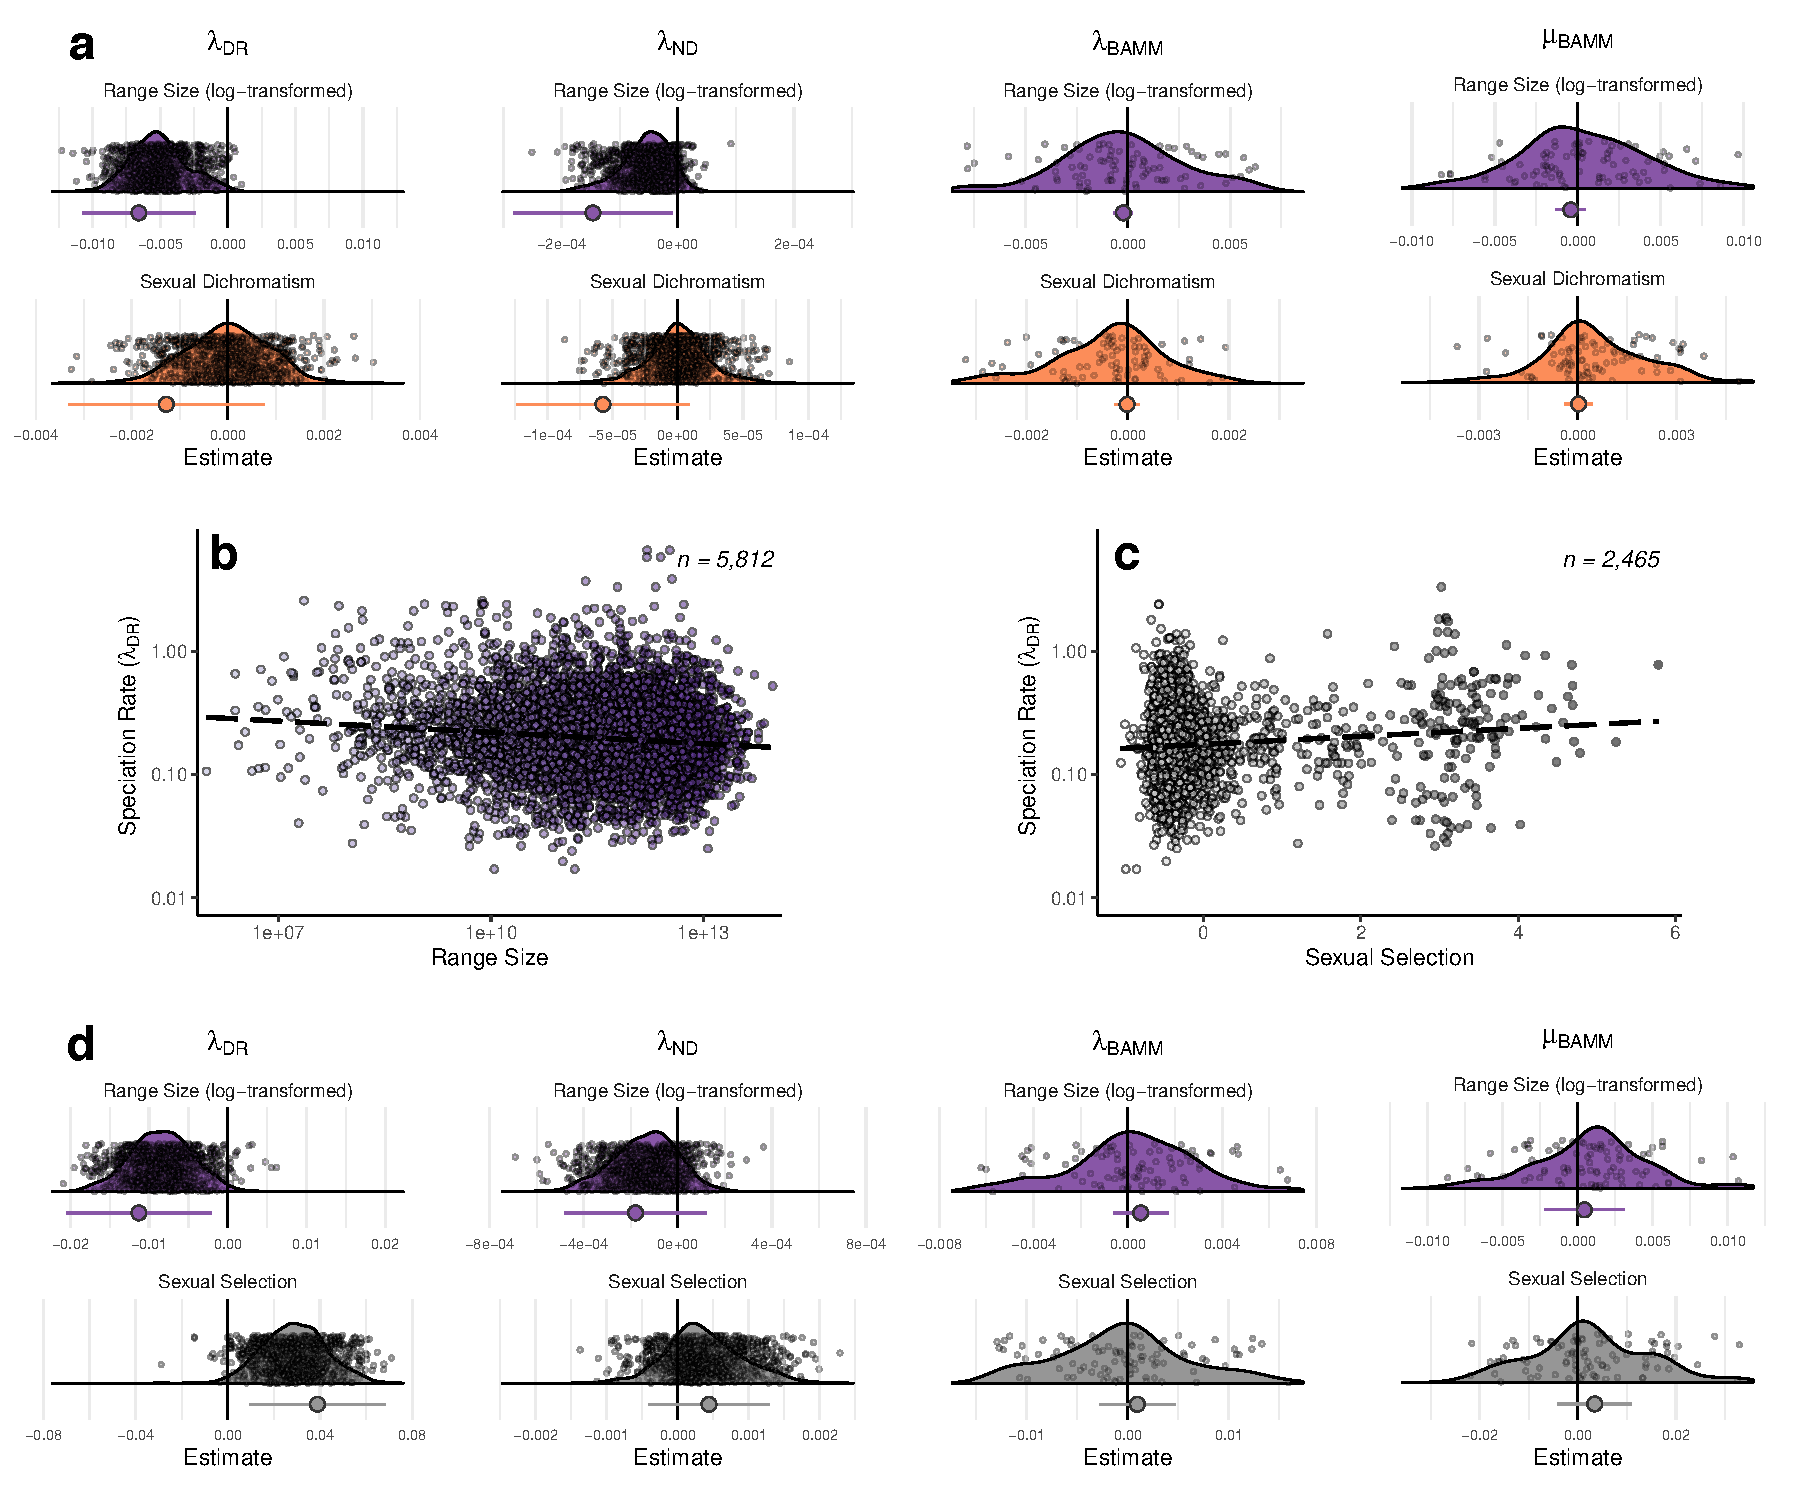
\includegraphics{Figures/Estimates_and_scatter_edit.pdf}
\caption{Model estimates (a) showing the effect size (i.e.~slope) of
log-range size and sexual dichromatism on speciation and extinction
rates using PGLS analyses with the sexual dichromatism dataset (RGB
values, \emph{n} = 5,812). (b) depicts the scatter plot of speciation
rate (\(\lambda_{DR}\)) and log-range size with the model estimate
presented as a dashed line. (c) shows the scatter plot of speciation
rate (\(\lambda_{DR}\)) and male-biased sexual selection (\emph{n} =
2,465). Similar to (a), (d) presents model estimates for PGLS analyses
using a restricted dataset with measures of an index of male-biased
sexual selection (\emph{n} = 2,465) and shows the effect of log-range
size and male-biased sexual selection on speciation and extinction
rates. Both datasets were used for analyses with three measures of
speciation (\(\lambda_{DR}\), \(\lambda_{ND}\), \(\lambda_{BAMM}\)) and
one measure of extinction (\(\mu_{BAMM}\)) as response variables. The
numerical values for the model estimates using the MCC tree and HPD
intervals of estimates from 1,000 randomly sampled trees (for
\(\lambda_{DR}\) and \(\lambda_{ND}\)) or 100 randomly sampled trees for
\(\lambda_{BAMM}\) and \(\mu_{BAMM}\) can be found in the Supplementary
Information. Density curves are based on model estimates from 1,000/100
trees and the circle below with error bars is the estimate and 95\% CIs
from the MCC tree. For this figure we removed outliers from estimates
coming from the 100 randomly sampled trees for BAMM models in order to
be able to visualise the MCC 95\% CIs. \label{model_results}}
\end{figure}

\begin{figure}
\centering
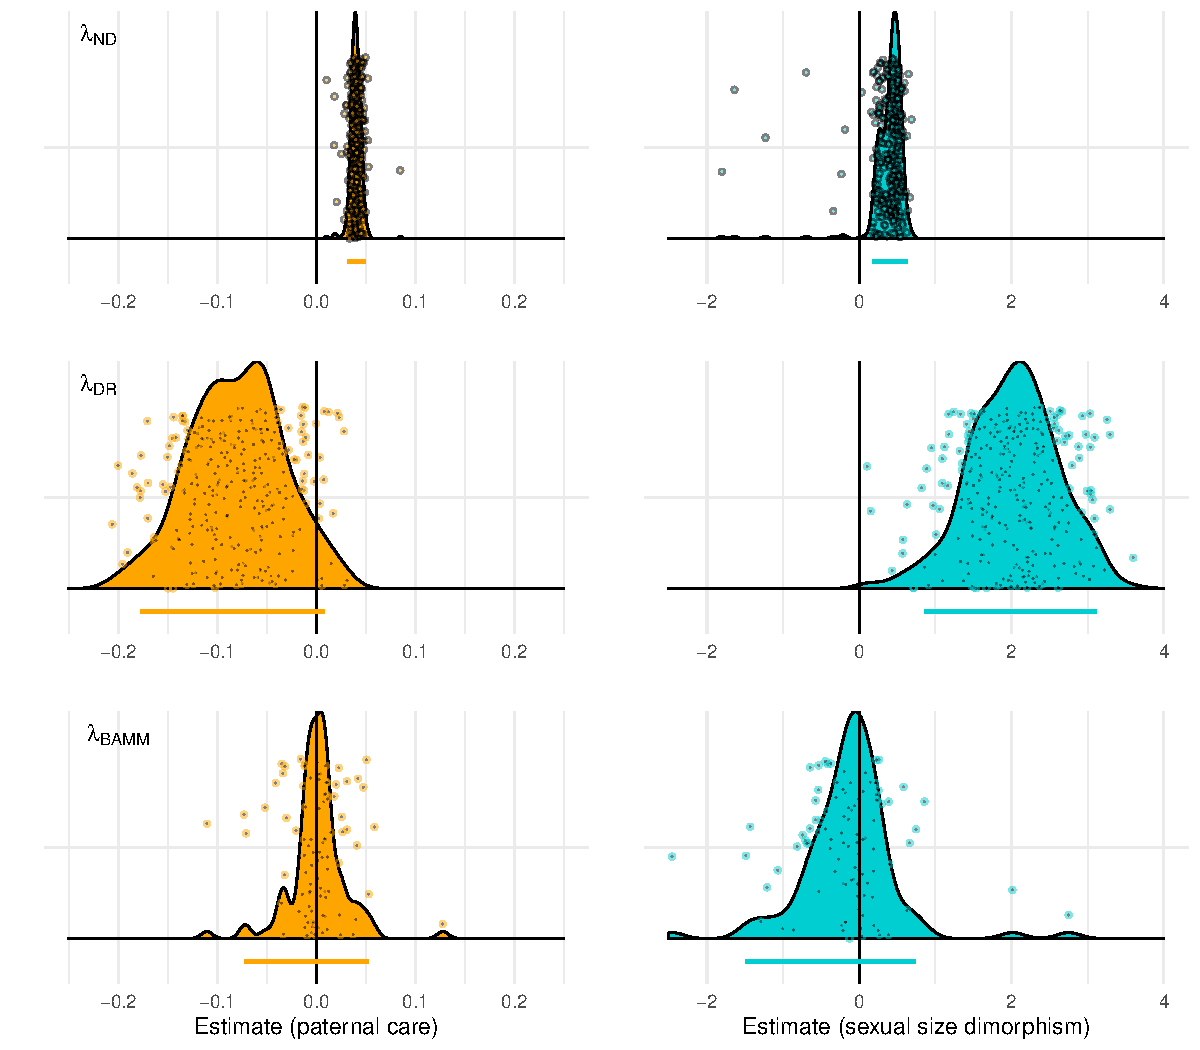
\includegraphics{Figures/Individual_SS_Estimates.pdf}
\caption{Estimates of the effect of individual sexual selection
components included in the PPCA (paternal care, sexual size dimorphism
and mating system) on three measures of speciation rate
(\(\lambda_{DR}\), \(\lambda_{ND}\) and \(\lambda_{BAMM}\)). Estimates
are presented as density intervals from pgls models on 300 phylogentic
trees that used species with available data for these sexual selection
measures (\emph{n} = 2,465). The bar under each density ridge is the 95
\% Highest Posterior Density Interval. Given that the mating system is a
categorical variable, model estimates for three polygynous mating system
levels are in reference to a striclty monogamous mating system (0\%
polygyny). \label{SS_components}}
\end{figure}

\begin{figure}
\centering
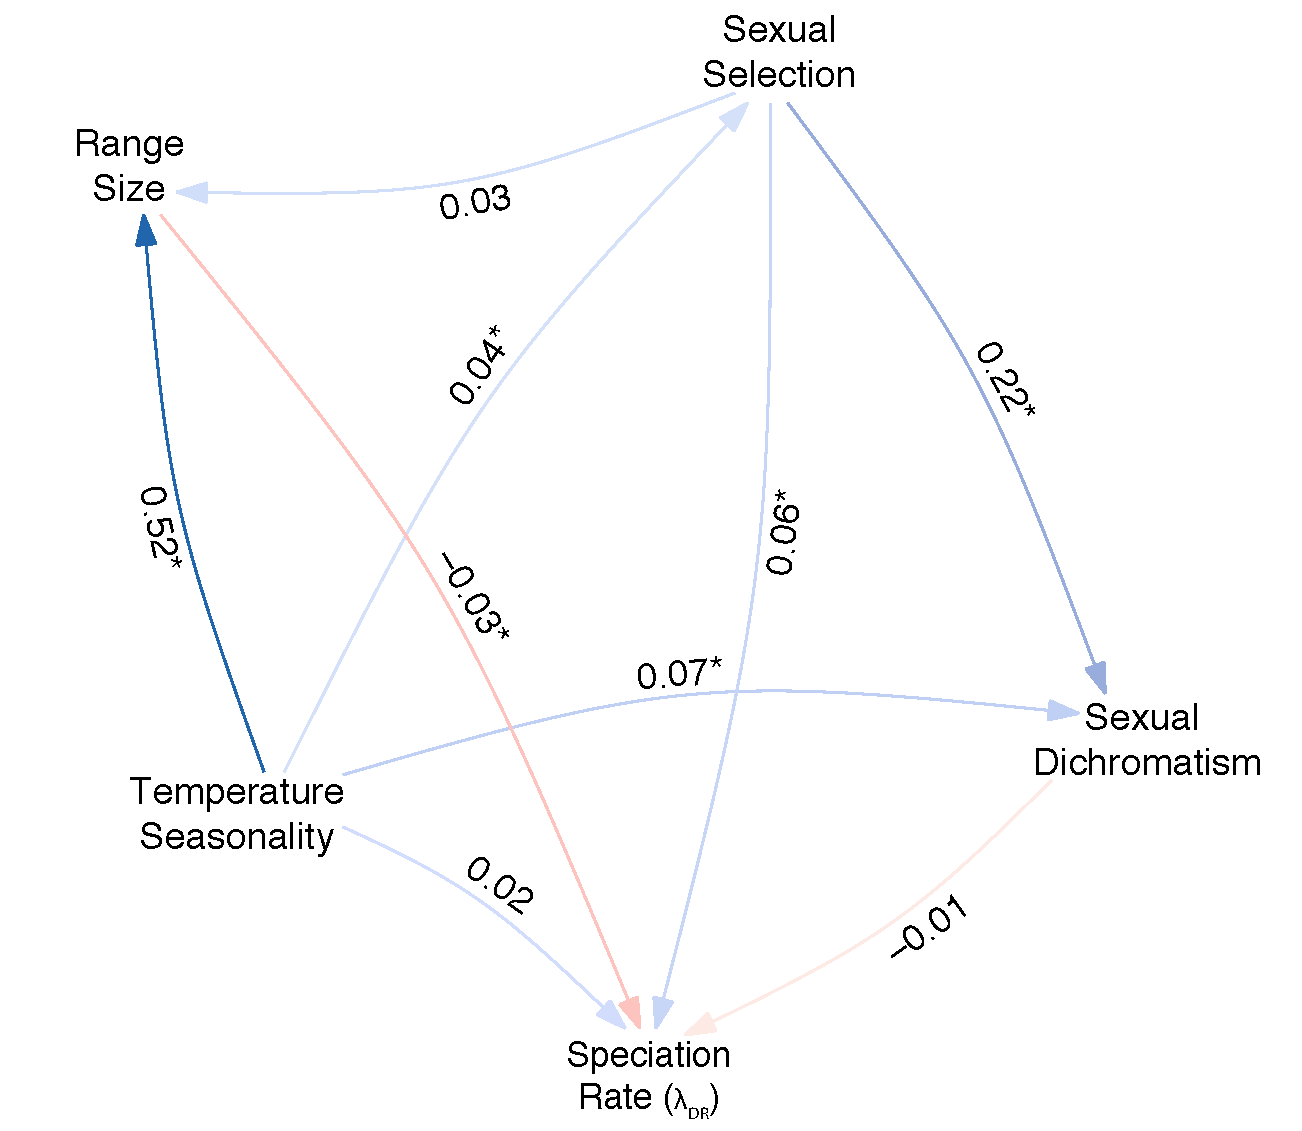
\includegraphics{Figures/Path_Analysis.pdf}
\caption{Path analysis of evolutionary and ecological variables. Arrows
represent direct effects with the direction of effect corresponding to
colours (blue = positive, red = negative). The numeric values are
standardised regression slopes and the asterisks indicates that the 95\%
confidence intervals of this estimate do not overlap with zero. The
confidence intervals were obtained from 500 bootstrapped iterations and
the data used in this analysis was subset to species with both sexual
dichromatism and an index of male-biased sexual selection measures
(\emph{n} = 2,465). \label{Path_Analysis}}
\end{figure}

\newpage\phantomsection

\hypertarget{discussion}{%
\section{Discussion}\label{discussion}}

We found evidence that the composite index of male-biased sexual
selection, but not measures of sexual dichromatism, is correlated with
the rate of speciation in passerine birds. The absence of a detectable
correlation between sexual dichromatism and speciation rate was
consistent across different measures of speciation (\(\lambda_{DR}\),
\(\lambda_{ND}\) and \(\lambda_{BAMM}\)) and both measures of
dichromatism (spectral and RGB), and it cannot be explained by a
difference in statistical power or sampling. These findings reaffirm the
conclusions of previous, smaller studies in which sexual dichromatism
was measured using spectrophotometry (Huang and Rabosky 2014) or human
observers (Cooney et al. 2017). The correlation between speciation rate
and the index of male-biased sexual selection (which encapsulates
variation in sexual size dimorphism, social polygyny, and paternal care)
was statistically significant for \(\lambda_{DR}\), but not for
\(\lambda_{ND}\) and \(\lambda_{BAMM}\). This pattern seems to be mainly
driven by an association between sexual size dimorphism and speciation.
Interestingly, we also found a consistent negative relationship between
range size and speciation rate, at least when this rate was quantified
using \(\lambda_{DR}\) and \(\lambda_{ND}\). None of the bioclimatic
measures of environmental variability that we investigated (i.e.,
temperature seasonality, long-term temperature variation, and spatial
temperature variation) were significantly associated speciation rate,
nor mediated the relationship between sexual selection and
diversification.

The difference in findings between the analyses of sexual dichromatism
\emph{versus} the index of male-biased sexual selection is noteworthy,
because the majority of earlier studies used dichromatism alone as their
proxy for sexual selection (e.g., Barraclough et al. 1995; Owens et al.
1999; Morrow et al. 2003; Seddon et al. 2013; Huang and Rabosky 2014).
Given our findings, and the modest correlation between dichromatism and
the sexual selection index (\(r = 0.34\); Dale et al. 2015), we suggest
that sexual dichromatism may not be a robust proxy for sexual selection
(Cooney et al. 2018). Although dichromatism almost certainly provides
some insight into the operation of sexual selection, it may be too
indirect a measure to detect any association with speciation rate, even
with large sample size. There are several reasons why the use of sexual
dichromatism as a proxy for sexual selection is problematic. Sexual
dichromatism can evolve for reasons other than sexual selection, such as
when males and females occupy different ecological niches (Wallace 1889;
Kottler 1980; Slatkin 1984; Shine 1989) or experience different
selective pressures in contexts other than competition for mates (Price
and Eaton 2014). For example, in superb fairy-wrens (\emph{Malurus
cyaneus}) female colouration has probably evolved in response to spatial
variation in predation pressure, increasing dichromatism (Medina et al.
2017). In fact, our path analysis detected a weak relationship between
environment and sexual dichromatism, where sexual dichromatism was
positively predicted by temperature seasonality (a measure of
environmental variation).

In line with some theoretical predictions and previous studies
(Kraaijeveld et al. 2011), we found that male-biased sexual selection
increases speciation rate, at least when speciation is measured by
\(\lambda_{DR}\). Many of the species that have both high scores of
male-biased sexual selection and high diversification rates belong to
the genera \emph{Ploceus}, \emph{Euplectes} (Ploceidae) and
\emph{Paradisaea} (Paradiaseidae). Multiple weaver species (Ploceidae)
are polygynous and lack paternal care, and both weavers and birds of
paradise have strong size dimorphism. The association between speciation
rates and principal component scores that we report seems to be mainly
driven by sexual size dimorphism and, to a lesser extent, paternal care.
Speciation rates (both \(\lambda_{DR}\) and \(\lambda_{ND}\)) are higher
in species with larger sexual dimorphism and \(\lambda_{DR}\) also has a
tendency to be higher in species with no paternal care. Size dimorphism
is often thought to arise as a consequence of intrasexual competition,
where one of the sexes (males in most birds) has to compete for access
to the other sex, leading to selection for larger body sizes and thus
greater dimorphism (Björklund 1990; Owens and Hartley 1998). Therefore,
competition between males could be the underlying driver of the high
speciation rates that we detect in some clades.

Sexual dimorphism due to competition within sexes contrasts with the
drivers of sexual dichromatism. Plumage dichromatism can evolve as a
consequence of female cryptic choice and be related to extra-pair
fertilizations, but not necessarily paternal care or mating system
(Owens and Hartley 1998). It can also arise as a result of selection on
the level of crypsis of the sex that cares for offspring (Dale et al.
2015). The fact that traits linked with competition (such as size
dimorphism) are the ones associated with higher \(\lambda_{DR}\) values
-- rather than sexual dichromatism -- supports the general view that
antagonistic interactions and sexual conflict can lead to increased
diversity (Bonduriansky 2011; Qvarnström et al. 2012; Tinghitella et al.
2018; Tsuji and Fukami 2020). Moreover, body size is a trait that
influences multiple aspects of the physiology and ecology of a species.
Differences in body size (as a result of sexual selection) could be
linked to changes in diet, vulnerability to predators or environmental
tolerance (Damuth 1993; Liow et al. 2008; Bonduriansky 2011), and such
differences could ultimately increase the likelihood of divergence
between young lineages. In mammals, sexual selection is suggested to
have driven the evolution of large body size which in turn has allowed
diversification of ecological strategies in the clade, and higher
speciation rates (McLain 1993; Bonduriansky 2011).

We also found that the association between sexual selection and
speciation appears to be independent of net primary productivity and
spatiotemporal variation in the environment. The lack of an effect of
these environmental variables on speciation rate has several possible
interpretations. Firstly, the effects of sexual selection on adaptation
and speciation may depend on the type of environmental variability under
which the species is evolving. Specifically, speciation rates might be
impacted by genetic constraints on adaptation, that vary across
environments. Theory suggests that sexual antagonism (which is often
exacerbated in species with strong sexual selection) may be lower in
habitats experiencing cyclical environmental variation
(e.g.~seasonality), relative to those experiencing directional change in
the environment (Connallon and Hall 2016). Another possibility is that
the environmental predictors we chose may not account for the key
ecological sources of selection that interact with sexual selection to
drive speciation. For example, our study does not include direct measure
of food availability or the severity of predation and parasitism, which
are both hypothesised to affect sexual selection and speciation
(reviewed in Maan and Seehausen 2011). Finally, it is possible that
environmental variability genuinely has little effect on speciation
rates, at least in the taxa investigated here.

We found that species with smaller ranges have elevated speciation
rates. This result is similar to a study of 329 amphibian genera, which
found higher diversification rates in taxa with smaller range size
(Greenberg and Mooers 2017). Intuitively, large range size should
promote speciation by creating more opportunities for geographic
barriers to form (Rosenzweig 1995; Castiglione et al. 2017). However,
the opposite pattern is also plausible because birds with limited
dispersal or more specialised niches can have more fragmented
populations, which would promote vicariant divergence and higher
speciation rates (Jablonski and Roy 2003; Birand et al. 2012; Claramunt
et al. 2012). Moreover, species that have recently split as a
consequence of vicariant divergence might have smaller ranges as a
result of the split of the ancestral lineage, leading to a link between
smaller ranges and shorter divergence times. It is also possible that
high speciation rates cause smaller range sizes, rather than the other
way around, for example because repeatedly-speciating lineages tend to
fill niches in ways that hinder the geographical expansion of new
species (Rosenzweig 1995; Weir and Price 2011; Price and Eaton 2014).
However, species undergoing adaptive radiation in new habitats are
unlikely to be limited by competition for resources from existing taxa.
One further explanation for the negative association between range size
and sexual dichromatism/sexual selection is the potential bias of
taxonomic classification, whereby over-splitting of species in clades
with large ranges leads to increased recent phylogenetic branching as
well as smaller ranges.

In addition to speciation, sexual selection is hypothesised to affect
extinction. Using the model-based approach of BAMM, we found no
association between the estimated extinction rate and sexual
dichromatism, male-biased sexual selection, or our measures of
environmental variability. However, these extinction results should not
be regarded as definitive because extinction is notoriously difficult to
estimate accurately from phylogenies, principally because different
combinations of speciation and extinction rates can give rise to similar
patterns of diversity (see Rabosky 2016). Phylogenetic methods such as
BAMM allow for speciation and extinction rates to be estimated using
moderately-sized phylogenies, although the ability of BAMM to model
evolutionary rate shifts and extinction rates is debated (see, Beaulieu
and O'Meara 2015; Rabosky 2016; Moore et al. 2016; Rabosky et al. 2017).
Additionally, while several tip-rate estimates exist for speciation rate
(e.g., \(\lambda_{DR}\) and \(\lambda_{ND}\)), tip-rate estimates of
extinction rate are difficult to obtain without complex Bayesian models
which are sensitive to sampling bias (Davis et al. 2013). Although
extinction rates can be inferred from alternative sources, such as the
fossil record (Martins et al. 2018), direct observation extinction, or
IUCN red list status (Greenberg and Mooers 2017), each approach has its
limitations. Across the passerine bird phylogeny, we found that BAMM
often produced homogeneous speciation and extinction rates for smaller
clades showing few rate shifts, which might reduce our power to detect
small differences in extinction rates among closely-related taxa
(Rabosky et al. 2017; Title and Rabosky 2018). Thus, this methodological
constraint likely decreases our ability to accurately measure the
correlation between metrics of sexual selection and the probability of
extinction.

One outcome of our analyses was that different measures of speciation
rates presented different results. This is not completely surprising,
because each of the rates is calculated differently (Title and Rabosky
2018). For instance, \(\lambda_{DR}\) is weighted more towards
speciation events close to the tips and allows more rate heterogeneity
compared to \(\lambda_{BAMM}\) estimates. Rate shifts are unlikely to be
detected in smaller clades in BAMM, meaning that it is not uncommon for
whole genera to have the same rate. Using the \(\lambda_{DR}\) metric,
only sister species are guaranteed to have the same rate. This leads to
greater variation in \(\lambda_{DR}\) relative to the \(\lambda_{BAMM}\)
estimates, which is suggested to be an advantage when studying
diversification patterns (Quintero et al. 2015). Additionally,
\(\lambda_{BAMM}\) estimates were more sensitive to phylogenetic
uncertainty and were 20 times more variable across trees compared to
\(\lambda_{DR}\) estimates. We cannot completely reject the idea that
the lack of association between \(\lambda_{BAMM}\) and sexual selection
could be the result of low statistical power, due to the combination of
both low variation across species in the speciation rates and high
levels of variation in the estimates across trees.

To summarise, we have shown that sexual size dimorphism (a putative
proxy for male-biased sexual selection), but not sexual dichromatism,
predicts speciation in passerines, that the magnitude of this effect is
modest, and that this relationship is not markedly affected by
environmental variability. We have also shown that there is no evidence
of an association between sexual selection and extinction rates.
Overall, our findings imply that male-male competition could be the
mechanism driving increased speciation rates in birds, that sexual
dichromatism may not be a reliable proxy for sexual selection, and that
alternative measures of sexual selection are more directly related to
diversification.

\phantomsection

\hypertarget{acknowledgements}{%
\section{Acknowledgements}\label{acknowledgements}}

We thank Adnan Moussalli for his assistance in conducting BAMM runs
across 100 phylogenetic trees, Ignacio Quintero for providing BAMM
results for comparison and for discussion of the results as well as
Chris Cooney for comments on the manuscript.

\phantomsection

\hypertarget{author-contributions}{%
\section{Author Contributions}\label{author-contributions}}

All authors contributed to conception, design and approach to analyses;
J.G.C. and J.D. compiled the data; J.G.C. and I.M. conducted analyses;
J.G.C. wrote the first draft of the manuscript; all authors contributed
substantially to further manuscript revisions.

\phantomsection

\hypertarget{data-accessibility}{%
\section{Data Accessibility}\label{data-accessibility}}

We have sought to make the data and Supplementary Material (including
\texttt{R} code) freely accessible to readers. The code and
Supplementary Material for this manuscript are available on
\href{https://justincally.github.io/SexualSelection_Speciation/}{GitHub}
and as an attached HTML document (Supplementary Material) for reviewers.
Data is archived in the adjoined GitHub repository and the environmental
dataset collated for this manuscript is available on Dryad:
\url{https://doi.org/10.5061/dryad.573n5tb6n}.

\newpage\phantomsection

\hypertarget{references}{%
\section{References}\label{references}}

\hypertarget{refs}{}
\leavevmode\hypertarget{ref-Armenta_2008}{}%
Armenta, J. K., P. O. Dunn, and L. A. Whittingham. 2008. Quantifying
avian sexual dichromatism: A comparison of methods. Journal of
Experimental Biology 211:2423.

\leavevmode\hypertarget{ref-Barraclough_1995}{}%
Barraclough, T. G., P. H. Harvey, and S. Nee. 1995. Sexual selection and
taxonomic diversity in passerine birds. Proceedings of the Royal Society
B-Biological Sciences 259:211--215.

\leavevmode\hypertarget{ref-MuMIn_2017}{}%
Bartoń, K. 2017. MuMIn: Multi-model inference.

\leavevmode\hypertarget{ref-Beaulieu_2015}{}%
Beaulieu, J. M., and B. C. O'Meara. 2015. Extinction can be estimated
from moderately sized molecular phylogenies. Evolution 69:1036--1043.

\leavevmode\hypertarget{ref-Belmaker_2015}{}%
Belmaker, J., and W. Jetz. 2015. Relative roles of ecological and
energetic constraints, diversification rates and region history on
global species richness gradients. Ecology Letters 18:563--571.

\leavevmode\hypertarget{ref-Berger_2014}{}%
Berger, D., K. Grieshop, M. I. Lind, J. Goenaga, A. A. Maklakov, and G.
Arnqvist. 2014. Intralocus sexual conflict and environmental stress.
Evolution 68:2184--2196.

\leavevmode\hypertarget{ref-Wouter_2018}{}%
Bijl, W. van der. 2018. \emph{Phylopath}: Easy phylogenetic path
analysis in R. PeerJ 6:e4718.

\leavevmode\hypertarget{ref-Birand_2012}{}%
Birand, A., A. Vose, and S. Gavrilets. 2012. Patterns of species ranges,
speciation, and extinction. American Naturalist 179:1--21.

\leavevmode\hypertarget{ref-birdlife_2017}{}%
BirdLife International and Handbook of the Birds of the World. 2017.
Bird species distribution maps of the world.
\url{http://datazone.birdlife.org/species/requestdis}.

\leavevmode\hypertarget{ref-bjorklund_1990}{}%
Björklund, M. 1990. A phylogenetic interpretation of sexual dimorphism
in body size and ornament in relation to mating system in birds. Journal
of Evolutionary Biology 3:171--183. Wiley Online Library.

\leavevmode\hypertarget{ref-Bonduriansky_2011}{}%
Bonduriansky, R. 2011. Sexual selection and conflict as engines of
ecological diversification. American Naturalist 178:729--745.

\leavevmode\hypertarget{ref-Bonduriansky_Chenoweth_2009}{}%
Bonduriansky, R., and S. F. Chenoweth. 2009. Intralocus sexual conflict.
Trends in Ecology \& Evolution 24:280--8.

\leavevmode\hypertarget{ref-Cally_2019}{}%
Cally, J. G., D. Stuart-Fox, and L. Holman. 2019. Meta-analytic evidence
that sexual selection improves population fitness. Nature communications
10:2017. Nature Publishing Group.

\leavevmode\hypertarget{ref-Candolin_2008}{}%
Candolin, U., and J. Heuschele. 2008. Is sexual selection beneficial
during adaptation to environmental change? Trends in Ecology \&
Evolution 23:446--452.

\leavevmode\hypertarget{ref-Castiglione_2017}{}%
Castiglione, S., A. Mondanaro, M. Melchionna, C. Serio, M. Di Febbraro,
F. Carotenuto, and P. Raia. 2017. Diversification rates and the
evolution of species range size frequency distribution. Frontiers in
Ecology and Evolution 5:147. Frontiers.

\leavevmode\hypertarget{ref-Claramunt_2012}{}%
Claramunt, S., E. P. Derryberry, J. V. Remsen, and R. T. Brumfield.
2012. High dispersal ability inhibits speciation in a continental
radiation of passerine birds. Proceedings of the Royal Society B:
Biological Sciences 279:1567.

\leavevmode\hypertarget{ref-Connallon_Hall_2016}{}%
Connallon, T., and M. D. Hall. 2016. Genetic correlations and
sex-specific adaptation in changing environments. 70:2198.

\leavevmode\hypertarget{ref-Cooney_2018}{}%
Cooney, C. R., H. E. A. MacGregor, N. Seddon, and J. A. Tobias. 2018.
Multi-modal signal evolution in birds: Re-examining a standard proxy for
sexual selection. Proceedings of the Royal Society of London B:
Biological Sciences 285.

\leavevmode\hypertarget{ref-Cooney_2017}{}%
Cooney, C. R., J. A. Tobias, J. T. Weir, C. A. Botero, and N. Seddon.
2017. Sexual selection, speciation and constraints on geographical range
overlap in birds. Ecology Letters 20:863--871.

\leavevmode\hypertarget{ref-Dale_2015}{}%
Dale, J., C. J. Dey, K. Delhey, B. Kempenaers, and M. Valcu. 2015. The
effects of life history and sexual selection on male and female plumage
colouration. Nature 527:367--370.

\leavevmode\hypertarget{ref-Damuth_1993}{}%
Damuth, J. 1993. Cope's rule, the island rule and the scaling of
mammalian population density. Nature 365:748--750. Nature Publishing
Group.

\leavevmode\hypertarget{ref-davies1986re}{}%
Davies, N., and A. Houston. 1986. Reproductive success of dunnocks,
\emph{Prunella modularis}, in a variable mating system. II. Conflicts of
interest among breeding adults. Journal of Animal Ecology 55:139--154.

\leavevmode\hypertarget{ref-Davis_2013}{}%
Davis, M. P., P. E. Midford, and W. Maddison. 2013. Exploring power and
parameter estimation of the BiSSE method for analyzing species
diversification. BMC Evolutionary Biology 13:38.

\leavevmode\hypertarget{ref-delhoyo2011}{}%
Del Hoyo, J., A. Elliott, and D. Christie. 2011. Handbook of the birds
of the world. Lynx Edicions 2003-2011.

\leavevmode\hypertarget{ref-dunn_2001}{}%
Dunn, P. O., L. A. Whittingham, and T. E. Pitcher. 2001. Mating systems,
sperm competition, and the evolution of sexual dimorphism in birds.
Evolution 55:161--175. Wiley Online Library.

\leavevmode\hypertarget{ref-Fick_2017}{}%
Fick, S. E., and R. J. Hijmans. 2017. WorldClim 2: New 1-km spatial
resolution climate surfaces for global land areas. International Journal
of Climatology 37:4302--4315.

\leavevmode\hypertarget{ref-Fromhage_2016}{}%
Fromhage, L., and M. D. Jennions. 2016. Coevolution of parental
investment and sexually selected traits drives sex-role divergence.
Nature Communications 7:12517.

\leavevmode\hypertarget{ref-Gomes_2016}{}%
Gomes, A. C. R., M. D. Sorenson, and G. C. Cardoso. 2016. Speciation is
associated with changing ornamentation rather than stronger sexual
selection. Evolution 70:2823--2838.

\leavevmode\hypertarget{ref-Greenberg_2017}{}%
Greenberg, D. A., and A. Ø. Mooers. 2017. Linking speciation to
extinction: Diversification raises contemporary extinction risk in
amphibians. Evolution Letters 1:40--48.

\leavevmode\hypertarget{ref-Hackett_2008}{}%
Hackett, S. J., R. T. Kimball, S. Reddy, R. C. K. Bowie, E. L. Braun, M.
J. Braun, J. L. Chojnowski, W. A. Cox, K.-L. Han, J. Harshman, C. J.
Huddleston, B. D. Marks, K. J. Miglia, W. S. Moore, F. H. Sheldon, D. W.
Steadman, C. C. Witt, and T. Yuri. 2008. A phylogenomic study of birds
reveals their evolutionary history. Science 320:1763--1768.

\leavevmode\hypertarget{ref-harano2010intralocus}{}%
Harano, T., K. Okada, S. Nakayama, T. Miyatake, and D. J. Hosken. 2010.
Intralocus sexual conflict unresolved by sex-limited trait expression.
Current Biology 20:2036--2039.

\leavevmode\hypertarget{ref-Harvey_2017}{}%
Harvey, M. G., G. F. Seeholzer, B. T. Smith, D. L. Rabosky, A. M.
Cuervo, and R. T. Brumfield. 2017. Positive association between
population genetic differentiation and speciation rates in new world
birds. Proceedings of the National Academy of Sciences 114:6328--6333.

\leavevmode\hypertarget{ref-Harvey_essim_2017}{}%
Harvey Michael, G., L. Rabosky Daniel, and N. Cooper. 2017. Continuous
traits and speciation rates: Alternatives to state‐dependent
diversification models. Methods in Ecology and Evolution 9:984--993.

\leavevmode\hypertarget{ref-Holman_Kokko_2013}{}%
Holman, L., and H. Kokko. 2013. The consequences of polyandry for
population viability, extinction risk and conservation. Philosophical
Transactions of the Royal Society B-Biological Sciences 368.

\leavevmode\hypertarget{ref-Hosner_2020}{}%
Hosner, P. A., H. L. Owens, E. L. Braun, and R. T. Kimball. 2020.
Phylogeny and diversification of the gallopheasants (aves: Galliformes):
Testing roles of sexual selection and environmental niche divergence.
Zoologica Scripta 49:549--562.

\leavevmode\hypertarget{ref-delhoyo_2016}{}%
Hoyo, J. del, and N. J. Collar. 2016. HBW and birdlife international
illustrated checklist of the birds of the world. Lynx Edicions; BirdLife
International.

\leavevmode\hypertarget{ref-Huang_2014}{}%
Huang, H. T., and D. L. Rabosky. 2014. Sexual selection and
diversification: Reexamining the correlation between dichromatism and
speciation rate in birds. American Naturalist 184:E101--E114.

\leavevmode\hypertarget{ref-Huber_2007}{}%
Huber, S. K., L. F. De Leon, A. P. Hendry, E. Bermingham, and J. Podos.
2007. Reproductive isolation of sympatric morphs in a population of
darwin's finches. Proceedings of the Royal Society of London B:
Biological Sciences 274:1709--1714.

\leavevmode\hypertarget{ref-Iglesias-Carrasco_2019}{}%
Iglesias-Carrasco, M., M. D. Jennions, S. Y. W. Ho, and D. A. Duchêne.
2019. Sexual selection, body mass and molecular evolution interact to
predict diversification in birds. Proceedings of the Royal Society B:
Biological Sciences 286:20190172.

\leavevmode\hypertarget{ref-Jablonski_2003}{}%
Jablonski, D., and K. Roy. 2003. Geographical range and speciation in
fossil and living molluscs. Proceedings of the Royal Society of London.
Series B: Biological Sciences 270:401--406. The Royal Society.

\leavevmode\hypertarget{ref-Janicke_2018}{}%
Janicke, T., M. G. Ritchie, E. H. Morrow, and L. Marie-Orleach. 2018.
Sexual selection predicts species richness across the animal kingdom.
Proceedings of the Royal Society B: Biological Sciences 285:20180173.
The Royal Society.

\leavevmode\hypertarget{ref-Jetz_2012}{}%
Jetz, W., G. H. Thomas, J. B. Joy, K. Hartmann, and A. O. Mooers. 2012.
The global diversity of birds in space and time. Nature 491:444--448.

\leavevmode\hypertarget{ref-Kokko_Brooks_2003}{}%
Kokko, H., and R. Brooks. 2003. Sexy to die for? Sexual selection and
the risk of extinction. Annales Zoologici Fennici 40:207--219.

\leavevmode\hypertarget{ref-Kokko_Jennions2008}{}%
Kokko, H., and M. D. Jennions. 2008. Parental investment, sexual
selection and sex ratios. Journal of Evolutionary Biology 21:919--948.

\leavevmode\hypertarget{ref-Kottler_1980}{}%
Kottler, M. J. 1980. Darwin, Wallace, and the origin of sexual
dimorphism. Proceedings of the American Philosophical Society
124:203--226.

\leavevmode\hypertarget{ref-Kraaijeveld_2011}{}%
Kraaijeveld, K., F. J. L. Kraaijeveld-Smit, and M. E. Maan. 2011. Sexual
selection and speciation: The comparative evidence revisited. Biological
Reviews 86:367--377.

\leavevmode\hypertarget{ref-Lande_1981}{}%
Lande, R. 1981. Models of speciation by sexual selection on polygenic
traits. Proceedings of the National Academy of Sciences 78:3721--3725.

\leavevmode\hypertarget{ref-Lande_1982}{}%
Lande, R. 1982. Rapid origin of sexual isolation and character
divergence in a cline. Evolution 36:213--223.

\leavevmode\hypertarget{ref-Liow_2008}{}%
Liow, L. H., M. Fortelius, E. Bingham, K. Lintulaakso, H. Mannila, L.
Flynn, and N. C. Stenseth. 2008. Higher origination and extinction rates
in larger mammals. Proceedings of the National Academy of Sciences
105:6097--6102. National Acad Sciences.

\leavevmode\hypertarget{ref-Long_2012}{}%
Long, T. A. F., A. F. Agrawal, and L. Rowe. 2012. The effect of sexual
selection on offspring fitness depends on the nature of genetic
variation. Current Biology 22:204--208.

\leavevmode\hypertarget{ref-Lorch_2003}{}%
Lorch, P. D., S. Proulx, L. Rowe, and T. Day. 2003. Condition-dependent
sexual selection can accelerate adaptation. Evolutionary Ecology
Research 5:867--881.

\leavevmode\hypertarget{ref-Maan_2011}{}%
Maan, M. E., and O. Seehausen. 2011. Ecology, sexual selection and
speciation. Ecology Letters 14:591--602.

\leavevmode\hypertarget{ref-Maia_2013}{}%
Maia, R., D. R. Rubenstein, and M. D. Shawkey. 2013. Key ornamental
innovations facilitate diversification in an avian radiation.
Proceedings of the National Academy of Sciences 110:10687--10692.
National Acad Sciences.

\leavevmode\hypertarget{ref-Martins_2018}{}%
Martins, M. J. F., T. M. Puckett, R. Lockwood, J. P. Swaddle, and G.
Hunt. 2018. High male sexual investment as a driver of extinction in
fossil ostracods. Nature 556:366.

\leavevmode\hypertarget{ref-Mason_2017}{}%
Mason, N. A., K. J. Burns, J. A. Tobias, S. Claramunt, N. Seddon, and E.
P. Derryberry. 2017. Song evolution, speciation, and vocal learning in
passerine birds. Evolution 71:786--796. Wiley Online Library.

\leavevmode\hypertarget{ref-Mclain_1993}{}%
McLain, D. K. 1993. Cope's rules, sexual selection, and the loss of
ecological plasticity. Oikos 490--500. JSTOR.

\leavevmode\hypertarget{ref-Medina_2017}{}%
Medina, I., K. Delhey, A. Peters, K. E. Cain, M. L. Hall, R. A. Mulder,
and N. E. Langmore. 2017. Habitat structure is linked to the evolution
of plumage colour in female, but not male, fairy-wrens. BMC evolutionary
biology 17:35.

\leavevmode\hypertarget{ref-Moore_2016}{}%
Moore, B. R., S. Hohna, M. R. May, B. Rannala, and J. P. Huelsenbeck.
2016. Critically evaluating the theory and performance of bayesian
analysis of macroevolutionary mixtures. Proceedings of the National
Academy of Sciences 113:9569--9574.

\leavevmode\hypertarget{ref-Morrow_Speciation_2003}{}%
Morrow, E. H., T. E. Pitcher, and G. Arnqvist. 2003. No evidence that
sexual selection is an 'engine of speciation' in birds. Ecology Letters
6:228--234.

\leavevmode\hypertarget{ref-Otto-Bliesner_2006}{}%
Otto-Bliesner, B. L., S. J. Marshall, J. T. Overpeck, G. H. Miller, A.
Hu, and. 2006. Simulating arctic climate warmth and icefield retreat in
the last interglaciation. Science 311:1751--1753.

\leavevmode\hypertarget{ref-Owens_1999}{}%
Owens, I. P. F., P. M. Bennett, and P. H. Harvey. 1999. Species richness
among birds: Body size, life history, sexual selection or ecology?
Proceedings of the Royal Society B-Biological Sciences 266:933--939.

\leavevmode\hypertarget{ref-owens_1998}{}%
Owens, I. P., and I. R. Hartley. 1998. Sexual dimorphism in birds: Why
are there so many different forms of dimorphism? Proceedings of the
Royal Society of London. Series B: Biological Sciences 265:397--407. The
Royal Society.

\leavevmode\hypertarget{ref-Pagel_1999}{}%
Pagel, M. 1999. Inferring the historical patterns of biological
evolution. Nature 401:877.

\leavevmode\hypertarget{ref-ape_2004}{}%
Paradis, E., J. Claude, and K. Strimmer. 2004. APE: Analyses of
phylogenetics and evolution in R language. Bioinformatics 20:289--290.

\leavevmode\hypertarget{ref-Pennell_2013}{}%
Pennell, T. M., and E. H. Morrow. 2013. Two sexes, one genome: The
evolutionary dynamics of intralocus sexual conflict. Ecology and
Evolution 3:1819--1834.

\leavevmode\hypertarget{ref-nlme_2018}{}%
Pinheiro, J., D. Bates, S. DebRoy, D. Sarkar, and R Core Team. 2018.
nlme: Linear and nonlinear mixed effects models.

\leavevmode\hypertarget{ref-Pischedda_2006}{}%
Pischedda, A., and A. K. Chippindale. 2006. Intralocus sexual conflict
diminishes the benefits of sexual selection. PLOS Biology 4:e356.

\leavevmode\hypertarget{ref-Price_2014}{}%
Price, J. J., and M. D. Eaton. 2014. Reconstructing the evolution of
sexual dichromatism: Current color diversity does not reflect past rates
of male and female change. Evolution 68:2026--2037.

\leavevmode\hypertarget{ref-Price-Waldman_2020}{}%
Price-Waldman, R. M., A. J. Shultz, and K. J. Burns. 2020. Speciation
rates are correlated with changes in plumage color complexity in the
largest family of songbirds. Evolution 74:1155--1169.

\leavevmode\hypertarget{ref-quintero_2018}{}%
Quintero, I., and W. Jetz. 2018. Global elevational diversity and
diversification of birds. Nature 555:246.

\leavevmode\hypertarget{ref-Quintero_2015}{}%
Quintero, I., P. Keil, W. Jetz, and F. W. Crawford. 2015. Historical
biogeography using species geographical ranges. Systematic Biology
64:1059--1073.

\leavevmode\hypertarget{ref-Qvarnstrom_2012}{}%
Qvarnström, A., N. Vallin, and A. Rudh. 2012. The role of male contest
competition over mates in speciation. Current Zoology 58:493--509.
Oxford University Press Oxford, Uk.

\leavevmode\hypertarget{ref-bammtools_2014}{}%
Rabosky, D., M. Grundler, C. Anderson, P. Title, J. Shi, J. Brown, H.
Huang, and J. Larson. 2014. BAMMtools: An R package for the analysis of
evolutionary dynamics on phylogenetic trees. Methods in Ecology and
Evolution 5:701--707.

\leavevmode\hypertarget{ref-Rabosky_2014}{}%
Rabosky, D. L. 2014. Automatic detection of key innovations, rate
shifts, and diversity-dependence on phylogenetic trees. PLOS ONE
9:e89543.

\leavevmode\hypertarget{ref-Rabosky_Extinction_2016}{}%
Rabosky, D. L. 2016. Challenges in the estimation of extinction from
molecular phylogenies: A response to Beaulieu and O'Meara. Evolution
70:218--228.

\leavevmode\hypertarget{ref-Rabosky_fish_2018}{}%
Rabosky, D. L., J. Chang, P. O. Title, P. F. Cowman, L. Sallan, M.
Friedman, K. Kaschner, C. Garilao, T. J. Near, M. Coll, and others.
2018. An inverse latitudinal gradient in speciation rate for marine
fishes. Nature 559:392.

\leavevmode\hypertarget{ref-Rabosky_BAMM_flawed_2017}{}%
Rabosky, D. L., J. S. Mitchell, and J. Chang. 2017. Is BAMM flawed?
Theoretical and practical concerns in the analysis of multi-rate
diversification models. Systematic biology 66:477--498.

\leavevmode\hypertarget{ref-Rankin_2011}{}%
Rankin, D. J., U. Dieckmann, and H. Kokko. 2011. Sexual conflict and the
tragedy of the commons. American Naturalist 177:780--791.

\leavevmode\hypertarget{ref-phytools_2012}{}%
Revell, L. J. 2012. Phytools: An r package for phylogenetic comparative
biology (and other things). Methods in Ecology and Evolution 3:217--223.

\leavevmode\hypertarget{ref-Rosenzweig_1995}{}%
Rosenzweig, M. L. 1995. Species diversity in space and time. Cambridge
University Press.

\leavevmode\hypertarget{ref-Safran_2013}{}%
Safran, R. J., E. S. Scordato, L. B. Symes, R. L. Rodrı'guez, and T. C.
Mendelson. 2013. Contributions of natural and sexual selection to the
evolution of premating reproductive isolation: A research agenda. Trends
in Ecology \& Evolution 28:643--650.

\leavevmode\hypertarget{ref-Seddon_2013}{}%
Seddon, N., C. A. Botero, J. A. Tobias, P. O. Dunn, H. E. A. MacGregor,
D. R. Rubenstein, J. A. C. Uy, J. T. Weir, L. A. Whittingham, and R. J.
Safran. 2013. Sexual selection accelerates signal evolution during
speciation in birds. Proceedings of the Royal Society B: Biological
Sciences 280.

\leavevmode\hypertarget{ref-Seddon_2008}{}%
Seddon, N., R. M. Merrill, and J. A. Tobias. 2008. Sexually selected
traits predict patterns of species richness in a diverse clade of
suboscine birds. American Naturalist 171:620--631.

\leavevmode\hypertarget{ref-Shine_1989}{}%
Shine, R. 1989. Ecological causes for the evolution of sexual
dimorphism: A review of the evidence. The Quarterly Review of Biology
64:419--461.

\leavevmode\hypertarget{ref-Slatkin_1984}{}%
Slatkin, M. 1984. Ecological causes of sexual dimorphism. Evolution
38:622--630.

\leavevmode\hypertarget{ref-sloan2019genitalia}{}%
Sloan, N. S., and L. W. Simmons. 2019. The evolution of female
genitalia. Journal of Evolutionary Biology in press.

\leavevmode\hypertarget{ref-swanson1998abalone}{}%
Swanson, W. J., and V. D. Vacquier. 1998. Concerted evolution in an egg
receptor for a rapidly evolving abalone sperm protein. Science
281:710--712.

\leavevmode\hypertarget{ref-Tinghitella_2018}{}%
Tinghitella, R. M., A. C. Lackey, M. Martin, P. D. Dijkstra, J. P.
Drury, R. Heathcote, J. Keagy, E. S. Scordato, and A. M. Tyers. 2018. On
the role of male competition in speciation: A review and research
agenda. Behavioral Ecology 29:783--797. Oxford University Press UK.

\leavevmode\hypertarget{ref-Rabosky_diversification_2018}{}%
Title, P. O., and D. L. Rabosky. 2018. Diversification rates and
phylogenies: What are we estimating, and how good are the estimates?
bioRxiv 369124.

\leavevmode\hypertarget{ref-tsuji2020sexual}{}%
Tsuji, K., and T. Fukami. 2020. Sexual dimorphism and species diversity:
From clades to sites. Trends in Ecology \& Evolution 35:105--114.
Elsevier.

\leavevmode\hypertarget{ref-Wallace_1889}{}%
Wallace, A. R. 1889. Colours and ornaments characteristic of sex.
\emph{in} Darwinism, an exponent of the theory of natural selection,
with some of its applications. Macmillan; Company.

\leavevmode\hypertarget{ref-Weir_2011}{}%
Weir, J. T., and T. D. Price. 2011. Limits to speciation inferred from
times to secondary sympatry and ages of hybridizing species along a
latitudinal gradient. American Naturalist 177:462--469.

\leavevmode\hypertarget{ref-west1983sexual}{}%
West-Eberhard, M. J. 1983. Sexual selection, social competition, and
speciation. Quarterly Review of Biology 58:155--183.

\leavevmode\hypertarget{ref-Whitlock_2000}{}%
Whitlock, M. C. 2000. Fixation of new alleles and the extinction of
small populations: Drift load, beneficial alleles, and sexual selection.
Evolution 54:1855--1861.

\leavevmode\hypertarget{ref-Whitlock_Agrawal_2009}{}%
Whitlock, M. C., and A. F. Agrawal. 2009. Purging the genome with sexual
selection: Reducing mutation load through selection on males. Evolution
63:569--582.

\leavevmode\hypertarget{ref-Zhao_2005}{}%
Zhao, M., F. A. Heinsch, R. R. Nemani, and S. W. Running. 2005.
Improvements of the modis terrestrial gross and net primary production
global data set. Remote Sensing of Environment 95:164--176.


\end{document}
